\chapter{Search for displaced leptons}
\label{displaced_leptons}
In this chapter, I present a search for new long-lived particles (LLPs) that could be produced in proton-proton collisions at a center-of-mass energy of \SI{13}{\TeV} at the LHC and detected by the CMS experiment. The search targets the unique signature of ``displaced leptons" that could be produced when LLPs decay to leptons after propagating a measurable distance from the location of the proton-proton collision. The candidate signal events include at least two leptons (one electron and one muon, two electrons, or two muons) whose transverse impact parameters are between \num{0.01} and \SI{10}{\cm}. Choosing transverse impact parameter as the main discriminating variable allows us to target pairs of displaced leptons without requiring that they form a common vertex. We apply an otherwise minimal event selection to retain sensitivity to a wide range of new physics models.

The Ohio State CMS group has previously performed two related searches for displaced leptons in the electron-muon final state: one in \SI{19.7}{\invfb} of \SI{8}{\TeV} data and another in \SI{2.6}{\invfb} of \SI{13}{\TeV} data~\cite{displaced_leptons_run1, displaced_leptons_bing}. The search presented here is the most sensitive to date. Some of the most significant improvements include:
\begin{itemize}
    \itemsep0em
    \item adding sensitivity to the electron-electron and muon-muon final states
    \item simplifying the event selection to reduce model dependence
    \item introducing a custom lepton isolation definition to significantly reduce the background from heavy-flavor meson decays
    \item implementing a new, fully data-driven background estimation procedure
    \item expanding the signal region to include leptons with smaller transverse impact parameters
    \item adding a second signal interpretation
    \item analyzing more than a factor of \num{40} times more data than the previous \SI{13}{\TeV} analysis~\cite{displaced_leptons_bing}
\end{itemize}

The ATLAS collaboration has also recently submitted a paper in which they target displaced leptons with transverse impact parameters between \num{0.3} and \SI{30}{\cm}. They observe no significant excess and set upper limits on the production cross section of long-lived sleptons in a gravity-mediated SUSY breaking model~\cite{atlas_displaced_leptons}.

The remainder of this chapter is organized as follows: Section~\ref{overview} introduces the displaced leptons experimental signature in the context of LLPs at the LHC and gives an overview of the analysis strategy, Section~\ref{samples} defines the data and simulated SM and signal samples used in the analysis, Section~\ref{selection} describes the event selection criteria and defines the signal and control regions, Section~\ref{corrections} describes the various corrections applied to the SM and signal simulation, Section~\ref{bg} investigates the sources of background and defines the procedure for estimating their contribution to the signal region, Section~\ref{systematics} describes the sources of systematic uncertainty in the efficiency for simulated signal events to pass the signal region selection, and Section~\ref{results} presents the results.

\section{Overview}
\label{overview}
\subsection{Long-lived particles at the LHC}
As discussed in Section~\ref{llps}, LLPs are common in the SM and naturally arise in many BSM scenarios. When produced in proton-proton collisions at the LHC, new LLPs have the potential to produce striking experimental signatures that differentiate them from SM backgrounds. As diagrammed in Fig.~\ref{llp_signatures}, new LLPs that decay within the detector volume can produce displaced vertices, physics objects whose trajectories do not point back to the location of the proton-proton collision, or particle tracks that vanish before reaching the outer edge of the tracker. Neutral LLPs that decay farther out can pass undetected through the tracker before producing signals in the calorimeters or muon system, and heavy, charged LLPs that are stable on detector length scales can be identified by their unusually large charge depositions.

\begin{figure}[hbtp]
\centering
\includegraphics[scale=0.4]{figures/overview/llp_signatures.pdf}
\caption{Illustration of several possible experimental signatures of long-lived particles. Image courtesy of Jamie Antonelli.} 
\label{llp_signatures}
\end{figure}

The identification of any of these LLP signatures above the expected background rates would be a clear sign of new physics, but their atypical nature adds an inherent layer of difficulty to studying such signatures. In fact, standard reconstruction algorithms and event selections frequently discard such unusual signatures and render the majority of LHC analyses insensitive to many BSM scenarios that include LLPs~\cite{llp_whitepaper}. As a solution to the naturalness problem may require new physics at the LHC energy scale, it is critical that physicists face the challenges posed by LLP analyses and look everywhere BSM physics may be hiding.

Interest in LLPs is growing as evidence of BSM physics continues to evade LHC physicists. Recent CMS searches in \SI{13}{\TeV} proton-proton collisions target disappearing tracks~\cite{disappearing_tracks} or use the ECAL timing capabilities to target photons or jets whose production at a displaced vertex delays the time of their detection~\cite{delayed_photons, delayed_jets}. All observations thus far agree with SM predictions, but these and other LLP analyses are probing regions of BSM parameter space that are untested by conventional analyses.

\subsection{Displaced leptons signature}
The Displaced Leptons analysis targets electrons and muons produced in the decays of new LLPs. Inspired by models such as Displaced SUSY (see Section~\ref{displaced_susy}), we take care to maintain sensitivity to leptons that are produced in separate long-lived decays as well as those that share a common displaced vertex. This goal is achieved by selecting pairs of leptons with large transverse impact parameters and setting no constraints on the presence or absence of displaced vertices. Figure~\ref{displaced_leptons_cartoon} shows the benefit of such an approach: the pair-produced new LLPs, labeled $X$, each decay to a single lepton and an unspecified second particle. The lepton transverse impact parameter, which is labeled $d_0$ in the figure and defined explicitly below, is then used to identify the displaced nature of the lepton decays without explicitly constraining the other decay products in any way. Note also that the same strategy would successfully identify two leptons from a single long-lived particle decay.

\begin{figure}
\centering
\includegraphics[width=0.7\textwidth]{figures/overview/signalEventDisplay.pdf}
\caption{Illustration of the displaced leptons signature showing the definition of $d_0$ in a transverse view of the CMS detector. $X$ denotes a new long-lived particle, $\ell$ denotes an electron or muon, and $Y$ denotes any other decay products of the new long-lived particle. When interpreting the results of the Displaced Leptons analysis with the Displaced SUSY model, $X$ refers to a top squark and $Y$ refers to a b or d quark.} 
\label{displaced_leptons_cartoon}
\end{figure}

Lepton transverse impact parameter, $d_0$, is defined as the distance of closest approach in the transverse plane of the helical trajectory of the lepton track to the CMS beamspot, which is the center of the region in which the proton bunches cross. $d_0$ is commonly measured with respect to the primary vertex, but in the case of leptons produced in displaced decays, the association between a given primary vertex and the resulting leptons is unreliable. We determine $d_0$ from measured properties of the lepton track using the following equation:
\begin{equation}
    d_0 = \frac{(v_x - x_0)p_y - (v_y - y_0)p_x}{\pt}
\end{equation}
where $v_x$ and $v_y$ refer to the $x$ and $y$ coordinates of the lepton track reference point, which is usually chosen to be the point of closest approach to the center of CMS, $x_0$ and $y_0$ refer to the $x$ and $y$ coordinates of the beamspot, and $p_x$, $p_y$, and \pt refer to the magnitudes of the $x$, $y$, and transverse components of the lepton's momentum. \ad is commonly used throughout the Displaced Leptons analysis because we generally care about the magnitude of $d_0$ but not its direction.

If we are to use lepton \ad as the discriminating variable in an LLP search, we must ensure it scales appropriately with the parent LLP lifetime. Typically, a particle with lifetime $\tau$ will travel a distance $d=\beta\gamma c \tau$, where $\beta$ and $\gamma$ are relativistic factors and $c$ is the speed of light, so $d$ and $\tau$ are directly correlated. Figure~\ref{displaced_leptons_cartoon} shows that lepton \ad is determined by the distance travelled by the new LLP in the transverse plane and the angle between the transverse momenta of the new LLP and the lepton. Unless this angle is pathologically constrained to zero, \ad and $\tau$ will be directly correlated as well. In fact, the maximum value of lepton \ad, which occurs when the angle between the transverse momenta of the new LLP and the lepton is $\frac{\pi}{2}$, is exactly equal to the transverse distance between the beamspot and location of the LLP decay.

Figure~\ref{d0_discriminating_power} shows the distribution of data and simulated Displaced SUSY events in the plane defined by electron and muon \ad. As expected, the data events, which are dominated by leptons from promptly decaying parent particles, are concentrated at low \ad values while the Displaced SUSY events are spread across the entire plane. This figure shows the power of \ad as a discriminating variable: requiring two leptons with $\ad>\SI{100}{\um}$ eliminates nearly all the SM background without requiring that the leptons form a common vertex.

\begin{figure}[hbtp]
\centering
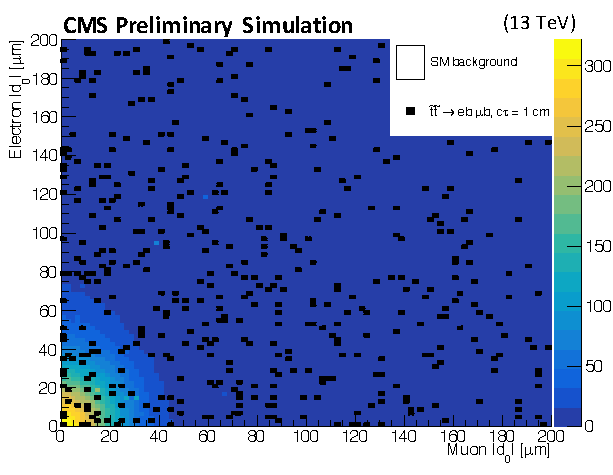
\includegraphics[scale=1.2]{figures/overview/d0_discriminating_power.pdf}
\caption{} 
\label{d0_discriminating_power}
\end{figure}
\fxnote{this is an ugly plot}

Another possible discriminating variable could be $\ad/\sigma_{\ad}$, where $\sigma_{\ad}$ is the uncertainty in \ad. Such a discriminating variable could potentially reduce the background from leptons with poorly measured \ad, but we choose to use \ad because of its straightforward correspondence to the parent particle lifetime. We also find that $\sigma_{\ad}$ is often underestimated, which reduces the potential benefit of using $\ad/\sigma_{\ad}$.

\subsection{Analysis strategy}
Having seen that \ad can be used to identify leptons from long-lived particle decays without requiring that the leptons form a common vertex, we now define a strategy to target such a signature. The basic analysis strategy is outlined here and described in detail in the following sections.

In addition to maximizing our sensitivity to models such as Displaced SUSY, we also strive to develop an analysis that is model independent, signature based, and easy to reinterpret. With these goals in mind, we perform a relatively simple cut-and-count analysis in which our main event selection sets no constraints on any non-lepton physics object. Unlike previous displaced leptons analyses~\cite{displaced_leptons_run1, displaced_leptons_bing}, we allow final states with more than two leptons and set no constraints on the lepton charge. As explained in Section~\ref{selection}, we select events in three analysis channels: electron-electron (\Pe\Pe), electron-muon (\Pe\Pgm), and muon-muon (\Pgm\Pgm). We then divide the events into different regions of the plane defined by the \ad of the two leptons that define the analysis channel. Figure~\ref{d0_discriminating_power}, for example, shows this plane in the $\Pe\Pgm$ channel. The signal region is defined as the region in which both leptons have $\ad>\SI{100}{\um}$.

Following the procedure defined in Section~\ref{bg}, we use the data in the non-signal regions to estimate the SM background in the signal region. Finally, we compare the background estimates and data yields in the signal region. In the absence of a significant excess, we use simulated signal events to constrain the available parameter space of the Displaced SUSY model. To avoid biasing the result, we blind ourselves to the data in the signal region and wait to observe the signal-region data until after we define and test the entire analysis procedure and receive pre-approval from the CMS Exotica Physics Analysis Group.

\pagebreak
\section{Data and simulated samples}
\label{samples}
\fxnote{add intro blurb?}
\subsection{Experimental data}
This analysis uses proton-proton collision data taken in 2016, 2017, and 2018 at a center-of-mass energy of \SI{13}{\TeV}. In 2016, we use only the last two run periods due to lower displaced tracking efficiency caused by an analog pipeline voltage saturation problem in the silicon strip detector during the earlier run periods (see appendix~\ref{k0}). In 2017, we use all run periods in the $\Pe\Pe$ channel and all but the earliest run period in the $\Pe\Pgm$ and $\Pgm\Pgm$ channels because the $\Pe\Pgm$ and $\Pgm\Pgm$ triggers are not available in the earliest run period. In 2018, we use all available run periods in all three channels. Ultimately, this analysis uses an integrated luminosity of \SI{16.1\pm0.4}{\fb} from 2016 in all three channels, \SI{41.5\pm1.0}{\fb} (\SI{36.7\pm0.8}{\fb}) from 2017 in the $\Pe\Pe$ channel ($\Pe\Pgm$ and $\Pgm\Pgm$ channels), and \SI{59.7\pm1.5}{\fb} from 2018 in all three channels.

The search is performed in the \texttt{MuonEG}, \texttt{DoubleEG} (in 2016--2017), \texttt{EGamma} (in 2018), and \texttt{DoubleMu} primary datasets. We also use the \texttt{MET} dataset to study the trigger efficiency and the \texttt{Cosmics} and \texttt{NoBPTX} datasets to study the displaced tracking efficiency. All data are reconstructed in the \texttt{07Aug17}, \texttt{31Mar2018}, \texttt{17Sep2018} reprocessing campaigns with software versions \texttt{CMSSW\_8\_0\_31}, \texttt{CMSSW\_9\_4\_8}, and \texttt{CMSSW\_10\_2\_0}, respectively. The sole exception is the \texttt{EGamma} 2018D dataset, which was reconstructed in the \texttt{22Jan2019} campaign. In all cases, we use the CMS \texttt{MiniAOD} event format.

\subsection{Simulated background events}
\label{bg_samples}
This analysis employs a fully data-driven background estimation technique that does not rely on simulated SM events. We do, however, use simulated SM events to study possible sources of background and verify the validity of the background estimation technique. The samples corresponding to 2016, 2017, and 2018 data conditions are from the \texttt{PdmVMCcampaignRunIISummer16}, \texttt{PdmVMCcampaignRunIIFall17}, and \texttt{PdmVMCcampaignRunIIAutumn18} production campaigns and were reconstructed in \texttt{CMSSW\_8\_0\_31}, \texttt{CMSSW\_9\_4\_8}, \texttt{CMSSW\_10\_2\_0} with the MiniAODSIM event format. The samples simulating $Z$+jets, $W$+jets, and \ttbar production are generated using \MGvATNLO~\cite{madgraph,fxfx,mlm}, while the samples simulating diboson ($WW$, $WZ$, and $ZZ$ with leptonic and semi-leptonic decays) and single-top-quark production are simulated with \POWHEG v2~\cite{Frixione:2002ik,Nason:2004rx,Frixione:2007vw,Alioli:2008gx,Alioli:2010xd}. \PYTHIA 8.2~\cite{PYTHIA8} is used to simulate the parton showering and hadronization for all processes. The modeling of the underlying event is generated using the CUETP8M1~\cite{Khachatryan:2015pea} and CP5 tunes~\cite{Sirunyan:2019dfx} for simulated samples corresponding to the 2016 and 2017--18 data sets, respectively.

\subsection{Simulated signal events}

We use simulated signal events to guide the analysis strategy and interpret our results. Samples of simulated $\Pp\Pp {\to} \PSQt \PASQt$ events in which the top squarks decay to a lepton and a $\cPqb$ quark or $\cPqd$ quark, are produced at leading order using \PYTHIA 8.2~\cite{PYTHIA8}. For simplicity, all lepton flavors are generated with equal branching fractions. The top squarks can form strongly-produced hadronic states called R-hadrons, which are generated with \PYTHIA. The interactions of the R-hadrons with matter are not simulated in \GEANTfour, but they are expected to have a negligible impact on the analysis because the lepton identification requirements effectively require the R-hadron to decay in the middle of the tracker volume. Each R-hadron therefore traverses $\lesssim1$ interaction length, making it unlikely to produce a high quality track, come to a stop in the detector, or flip its charge. To generate the samples, we start with a SUSY Les Houches Accord file~\cite{LesHouches} corresponding to Snowmass Points and Slopes point 1a~\cite{snowmass_points_slopes} and modify the mass and width of the top squark according to the sample being produced. We generate samples with $\PSQt$ masses from \num{100} to \SI{1800}{\GeV} at \SI{100}{\GeV} intervals and with $\PSQt$ lifetimes at each decade from \SI{0.1}{\mm} to \SI{1}{m}. After producing these samples, we also employ a lifetime reweighting technique to effectively produce eight additional lifetime points between each pair of adjacent lifetimes. In the case of the 1~m samples, we also use an equivalent technique to effectively produce nine additional lifetime points between \num{1} and \SI{10}{\m}. The production cross sections for each $\PSQt$ mass hypothesis are taken from the website of the LHC SUSY Cross Section Working Group. The signal samples are reconstructed in the same campaigns and with the same conditions as the SM background samples described in \ref{bg_samples}.
\fxnote{cite something for the xs or add a table or both}

\fxnote{In addition to the signal samples described above, we also interpret our results with $\Pp\Pp \to \sLep\sLepbar \to \PAl\PXXSG\:\Pl\PXXSG$ and $\Pp\Pp \to \PH \to \mathrm{S}\mathrm{S} \to \Pl\PAl\:\Pl\PAl$ processes. The simulated $\Pp\Pp \to \sLep\sLepbar \to \PAl\PXXSG\:\Pl\PXXSG$ samples are generated at leading order using \MGvATNLO, and the simulated $\Pp\Pp \to \PH \to \mathrm{S}\mathrm{S} \to \Pl\PAl\:\Pl\PAl$  samples are generated using \POWHEG v2 and \PYTHIA 8.2 at next-to-leading order.}

\pagebreak
\section{Event selection}
\label{selection}
\fxnote{add intro blurb?}
\subsection{Triggers}
The events are required to pass different triggers in each channel. Standard CMS electron and muon triggers are not designed for displaced objects, so we use nonstandard triggers for both electrons and muons. For muons, we remove all trigger requirements relating to the muon $d_0$, longitudinal impact parameter ($d_z$), or the vertex from which the muon originates. For electrons, we actually use photon triggers, which collect events with electrons as well as photons but do not rely on any tracking information. See Section~\ref{trigger} for a brief overview of the CMS trigger system.

In the \Pe\Pgm\ channel, 2016 data and corresponding simulated events are required to pass the logical OR of two HLT paths (\longvar{HLT_Mu38NoFiltersNoVtx_Photon38_CaloIdL_v*} OR \longvar{HLT_Mu28NoFiltersNoVtxDisplaced_Photon28_CaloIdL_v*}) that were both originally designed for the 2015 CMS displaced leptons analysis~\cite{displaced_leptons_bing}. The first trigger requires at least one muon with $\pt>\SI{38}{\GeV}$ and places no constraints on the vertex, $d_0$, or $d_z$. The second trigger requires at least one muon with $\pt>\SI{28}{\GeV}$ and $\ad>\SI{0.01}{\cm}$. Each of these two triggers also requires at least one photon that passes a loose calorimeter-based identification. The first (second) trigger requires that the photon \ET is greater than \SI{38}{\GeV} (\SI{28}{\GeV}). The signal efficiency with these dedicated triggers is significantly higher than that of standard muon-photon HLT paths.

In 2017 and 2018, data and corresponding simulated events in the \Pe\Pgm\ channel are required to pass \longvar{HLT_Mu43NoFiltersNoVtx_Photon43_CaloIdL_v*}. The muon \pt and photon \ET thresholds are raised with respect to 2016 due to increased pileup. A version of the 2016 trigger that requires displaced muons is not available in 2017 and 2018.

In the \Pe\Pe\ channel, 2016 data and corresponding simulated events are required to pass the logical OR of two HLT paths (\longvar{HLT_Diphoton30_18_R9Id_OR_IsoCaloId_AND_HE_R9Id_Mass90_v*} OR  \longvar{HLT_DoublePhoton60_v*}). The first requires a leading photon with $\ET>30\GeV$ and a subleading photon with $\ET>\SI{18}{\GeV}$. Photons must pass calorimeter identification criteria involving isolation, the ratio of HCAL to ECAL energy, and shower shape, and the di-photon invariant mass must be $>\SI{90}{\GeV}$. This path is highly efficient at low top squark mass. The second trigger simply requires at least two photons with $\ET>\SI{60}{\GeV}$. This path is highly efficient at large top squark mass and lifetime.

In 2017 and 2018, data and corresponding simulated events in the \Pe\Pe\ channel are required to pass \longvar{HLT_Diphoton30_22_R9Id_OR_IsoCaloId_AND_HE_R9Id_Mass90_v*} OR  \longvar{HLT_DoublePhoton70_v*}. The photon \ET thresholds are raised with respect to 2016 due to increased pileup.

In the \Pgm\Pgm\ channel, 2016 data and corresponding simulated events are required to pass the logical OR of two HLT paths (\longvar{HLT_DoubleMu33NoFiltersNoVtx_v*} OR \longvar{HLT_DoubleMu23NoFiltersNoVtxDisplaced_v*}) that were both designed for this analysis. The first trigger requires at least two muons with $\pt>\SI{33}{\GeV}$ and sets no constraints on the vertex, $d_0$, or $d_z$. The second trigger requires at least two muons with $\pt>\SI{23}{\GeV}$ and $\ad>\SI{0.01}{\cm}$. The signal efficiency with these dedicated triggers is significantly higher than that of standard di-muon HLT paths.

In 2017 and 2018, data and corresponding simulated events in the \Pgm\Pgm\ channel are required to pass \longvar{HLT_DoubleMu43NoFiltersNoVtx_v*}. The muon \pt threshold is raised with respect to 2016 due to increased pileup. A version of the 2016 trigger that requires displaced muons is not available in 2017 and 2018.

\subsection{Preselection}
\label{preselection}
Starting from the events collected with the triggers described above, we next apply a set of preselection criteria to select the events to be analyzed. The preselection criteria vary by channel and year, but the fundamental goal is always to select events with at least one good reconstructed lepton of each flavor required by the channel. 

Specifically, the \Pe\Pgm\ preselection selects events with at least one PF electron and at least one global PF muon, the \Pe\Pe\ preselection selects events with at least two PF electrons, and the \Pgm\Pgm\ preselection selects events with at least two global PF muons (see Section~\ref{cms_reco} for a discussion of the PF algorithm). We set requirements on these electrons and muons as shown in Tables~\ref{preselection_emu}, \ref{preselection_ee}, and \ref{preselection_mumu}. The electron and muon \pt  requirements are chosen such that the trigger efficiency is independent of lepton \pt,\fxnote{reference trig eff section after adding trig eff plots} while electron and muon $\abs{\eta}$ requirements are chosen to reduce the fraction of leptons with poorly measured $d_0$ (see Appendix~\ref{large_eta}). Electrons that traverse the gap between the endcap and barrel detectors are also rejected due to the known decrease in reconstruction performance in this region.

\begin{sidewaystable}
\noindent \centering{}
\topcaption{The $\Pe\Pgm$ preselection criteria. The electron and muon \pt thresholds increase in 2017 in accordance with the increased HLT electron and muon \pt thresholds.}
\label{preselection_emu}
\begin{tabular}{lll}
\hline
\multicolumn{3}{c}{Object-level selections} \\
Selection variable & Electron     & Muon \\
\hline 
Number             & $\geq1$         & $\geq1$\\[2mm]
\multirow{2}{*}{\pt}& $>42\GeV$ (2016)    & $>40\GeV$ (2016)\\
                & $>45\GeV$ (2017 and 2018)    & $>45\GeV$ (2017 and 2018)\\[2mm]
$\abs{\eta}$           & $<1.5$      & $<1.5$\\[2mm]
 & not in ECAL gap & -\\[2mm]
\multirow{2}{*}{$\eta-\phi$}& veto ($1.0<\eta<1.5$ and $\phi>2.7$) (2017)    & veto ($1.0<\eta<1.5$ and $\phi>2.7$) (2017)\\
                & veto ($0.3<\eta<1.2$ and $0.4<\phi<0.8$) (2018)   & veto ($0.3<\eta<1.2$ and $0.4<\phi<0.8$) (2018)\\[2mm]
ID                 & Tight (cut-based) & Tight (cut-based)\\[2mm]
Custom isolation   & Tight        & Tight \\
\hline
\hline
\multicolumn{3}{c}{Event-level selections}\\
\hline
\multicolumn{3}{c}{Zero $\Pgm\Pgm$ pairs with $\cos{\alpha}<-0.99$} \\
\multicolumn{3}{c}{Reject $\Delta t<-20\ns$, if both timing ndof$>7$} \\
\multicolumn{3}{c}{At least one $\Pe\Pgm$ pair with $\DR(\Pe,\Pgm)>0.2$} \\
\multicolumn{3}{c}{Reject events with candidate leptons form a displaced vertex in the tracker material} \\
\hline
\end{tabular}
\end{sidewaystable}
\begin{sidewaystable}
\setlength{\tabcolsep}{40pt}
\noindent \centering{}
\topcaption{The $\Pe\Pe$ preselection criteria. The electron \pt threshold increased in 2017 and 2018 because the HLT electron \pt threshold increased at the start of 2017.}
\label{preselection_ee}
\begin{tabular}{ll}
\hline
\multicolumn{2}{c}{Object-level selections}\\
Selection variable & Electron          \\
\hline
Number               & $\geq2$              \\[2mm]
\multirow{2}{*}{\pt} & $>65\GeV$ (2016)\\
                     & $>75\GeV$ (2017 and 2018)\\[2mm]
$\abs{\eta}$             & $<1.5$\\[2mm]
                     & not in ECAL gap\\[2mm]
\multirow{2}{*}{$\eta-\phi$ (pixel power supply issue)}& veto ($1.0<\eta<1.5$ and $\phi>2.7$) (2017)\\
                & veto ($0.3<\eta<1.2$ and $0.4<\phi<0.8$) (2018)\\[2mm]
ID                   & Tight (cut-based) \\[2mm]
Custom isolation     & Tight             \\
\hline
\hline
\multicolumn{2}{c}{Event-level selections}\\
\hline
\multicolumn{2}{c}{At least one $\Pe\Pe$ pair with $\DR(\Pe,\Pe)>0.2$} \\
\multicolumn{2}{c}{Reject events where the candidate electrons form a good displaced vertex that overlaps with the tracker material} \\
\multicolumn{2}{c}{Reject events with displaced muons in the $\Pe\Pgm$ channel inclusive signal region} \\
\hline
\end{tabular}
\end{sidewaystable}
\input{tables/preselection_mumu}

We use a tight cut-based identification (ID) on the electrons and muons to select well-reconstructed leptons, but unlike the standard ID definitions used in many CMS analyses, we do not place any requirements on $d_0$ or $d_z$. In all other respects, we follow the cut-based ID recommendations of the CMS EGamma and Muon Physics Object Groups. The electron ID corresponds to \longvar{egmGsfElectronIDs:cutBasedElectronID-Summer16-80X-V1-tight} in 2016, \longvar{egmGsfElectronIDs:cutBasedElectronID-Fall17-94X-V1-tight} in 2017, and \longvar{egmGsfElectronIDs:cutBasedElectronID-Fall17-94X-V2-tight} in 2018. The electron and muon tight ID requirements are summarized in Tables \ref{e_tight_id} and \ref{tab:mu_tight_id}.

\begin{table}
\noindent \centering{}
\topcaption{The electron tight ID requirements, which are identical to the tight cut-based ID from the CMS EGamma Physics Object Group with the $d_0$ and $d_z$ requirements removed. Electron ID quantity definitions are available in Ref.~\cite{electron_performance_run1}.}
\label{e_tight_id}
\begin{tabular}{ll}
\hline
Electron ID requirements\\
\hline 
\multirow{2}{*}{full5x5 $\sigma_{i\eta i\eta} <$}     & 0.0104 (2018, 2017)                \\
                                                     & 0.00998 (2016)                     \\[2mm]
\multirow{3}{*}{$|\delta\eta_{\mathrm{Seed}}| < $}     & 0.00255 (2018)                     \\
                                                     & 0.00353 (2017)                     \\
                                                     & 0.00308 (2016)                     \\[2mm]
\multirow{3}{*}{$|\delta\phi_{\mathrm{In}}| < $}       & 0.022 (2018)                       \\
                                                     & 0.0499 (2017)                      \\
                                                     & 0.0816 (2016)                      \\[2mm]
\multirow{3}{*}{$\mathrm{H/E} <$}                    & $0.026+1.15/\mathrm{E}+0.0324\rho/\mathrm{E}$ (2018)  \\
& $0.026+1.12/\mathrm{E}+0.0368\rho/\mathrm{E}$ (2017)  \\
& 0.0414 (2016)  \\[2mm]
\multirow{3}{*}{PF isolation $<$}  & $0.0287+0.506/\pt$ (2018)         \\
                                                     & 0.0361 (2017)          \\
                                                     & 0.0588 (2016)          \\[2mm]
\multirow{3}{*}{$|1/\mathrm{E}-1/\mathrm{p}|<$}   & 0.159 (2018)              \\
                                                  & 0.0278 (2017)             \\
                                                  & 0.0129 (2016)             \\[2mm]
expected missing inner hits $<=$ & 1                            \\[2mm]
pass conversion veto	         & yes                          \\[2mm]
\hline
\end{tabular}
\end{table}
\begin{table}
\noindent \centering{}
\topcaption{The muon tight ID requirements. They are identical to the tight cut-based ID from the muon Physics Object Group, except we remove any requirements on $d_0$ or $d_z$~\cite{muonPOGtightID}.}
\label{tab:mu_tight_id}
\begin{tabular}{ll}
\hline
Muon ID requirements\\
\hline 
Is a global muon\\
Is a PF muon\\
$\chi^{2}/\mathrm{n_{dof}}$ of the global-muon track fit is $<10$\\
At least one muon-chamber hit included in the global-muon track fit\\
Muon segments in at least two muon stations\\
At least 1 valid pixel hit\\
At least 6 tracker layers with hits\\
\hline
\end{tabular}
\end{table}

We also require that electrons and muons are isolated. Specifically, we use a modified isolation definition that accounts for the fact that displaced leptons may be associated with the wrong primary vertex. The standard PF isolation assumes all energy from primary vertices other than the leading primary vertex is due to pileup, which is not true when the primary vertex ordering is altered by an incorrectly associated lepton. We have therefore modified the isolation definition to be agnostic to the primary vertex ordering by allowing PF candidates from any primary vertex to contribute to the isolation sum and by using a simple $\rho$-based pileup correction, where $\rho$ is the total transverse energy of all the PF candidates in an event divided by the total detector area. The modified isolation is calculated as:
\begin{equation}
    \text{relative isolation} = \frac{\text{max}\left(0,\ \pt^{h^{\pm}} + \ET^{h^0} + \ET^{\Pgg} - \rho\pi R^2\right)}{\pt^{\ell}}
\end{equation}
where $R$ is the radius of a cone in the $\eta$-$\phi$ plane that is centered on the lepton, $\pt^{h^{\pm}}$ is the total \pt of charged hadrons in the cone, $\ET^{h^0}$ is the total \ET of neutral hadrons in the cone, $\ET^{\Pgg}$ is the total contribution of photons in the cone, $\rho$ is defined as above, and $\pt^{\ell}$ is the lepton \pt. R is set to \num{0.3} for electrons and \num{0.4} for muons.

Figure~\ref{iso_pu_term_comparison} shows how the size of the pileup correction term depends on lepton displacement in the standard isolation but not in the modified isolation described here. We use the modified isolation definition for both electrons and muons while keeping the original tight working point for electrons and slightly tightening the tight working point for muons. In the end, we require that the relative isolation is $<0.10$ for muons and $<0.0588$ for electrons in 2016 and $<0.0287+0.506/\pt$ for electrons in 2017 and 2018. As shown in Figs.~\ref{iso_performance_comparison} and \ref{iso_signal_bg}, this modified PF isolation rejects substantially more background when the leptons are displaced but does not significantly alter the signal yield. We note, however, that there may still be some minor dependence on the primary vertex selection in the PF muon requirement because the PF muon selection includes some loose isolation requirements where the charged hadron component is constrained to the selected primary vertex.

\begin{figure}
\centering
\includegraphics[width=0.44\textwidth]{figures/selection/CustomVsStandardMuIsoPUcorrection_2018emuTTbar_PCR.png}
\includegraphics[width=0.45\textwidth]{figures/selection/CustomVsStandardMuIsoPUcorrection_2018emuTTbar_500To1000um.png}
\caption{The muon isolation pileup correction term, for the standard muon isolation and the modified muon isolation in simulated \ttbar events that pass the $\Pe\Pgm$ preselection in 2018 conditions. The plot on the left is for muon $\ad<\SI{100}{\um}$, and the plot on the right is for muon $500<\ad<\SI{1000}{\um}$.}
\label{iso_pu_term_comparison}
\end{figure}

\begin{figure}\fxnote{weirdly low resolution}
\centering
\includegraphics[width=0.45\textwidth]{figures/selection/StandardIso_ElectronD0vsMuonD0_2018emuTTbar.png}
\includegraphics[width=0.44\textwidth]{figures/selection/CustomIso_ElectronD0vsMuonD0_2018emuTTbar.png}
\caption{The electron \ad versus the muon \ad, for \ttbar simulated events that pass the $\Pe\Pgm$ preselection and where at least one lepton comes from a heavy-flavor meson. The plot on the left uses the standard isolation, and the plot on the right uses the modified isolation.}
\label{iso_performance_comparison}
\end{figure}

\begin{figure}\fxnote{weirdly low resolution}
\centering
\includegraphics[width=0.5\textwidth]{figures/selection/MuonCustomIso_TTbar_Signal.png}
\caption{The muon custom isolation distribution for simulated \ttbar background and \stoptolb signal events in 2018 conditions\fxnote{specify selection}.}
\label{iso_signal_bg}
\end{figure}

We also reject electrons and muons in certain regions of the $\eta$-$\phi$ plane where lepton $d_0$ is more likely to be mismeasured. We identify these regions as highly populated bins in the electron $\eta$-$\phi$ distribution in a prompt-muon, displaced-electron control region in 2017 and 2018 data (see Fig.\ref{eta_phi_vetos}). No such bins are present in 2016 data. The identified regions coincide with regions found by a previous CMS analysis~\cite{disappearing_tracks} to be affected by power supply issues in the pixel detector. The $\eta$-$\phi$ variation is more apparent for displaced electrons than displaced muons, so we use data in a prompt muon ($\ad<\SI{40}{\um}$), displaced electron ($\num{100}<\ad<\SI{500}{\um}$) control region to define the  regions used for both electrons and muons. In 2017, the rejected region is $1.0<\eta<1.5$ AND $\phi>2.7$, and in 2018 the rejected region is $0.3<\eta<1.2$ AND $0.4<\phi<0.8$.

\begin{figure}
\centering
\includegraphics[scale=0.3]{figures/selection/displacedE_etaPhi_data_2017.pdf}
\includegraphics[scale=0.3]{figures/selection/displacedE_etaPhi_data_2018.pdf}
\caption{The electron $\eta-\phi$ distribution in a prompt-muon, displaced-electron control region\fxnote{define quantitatively?} in 2017 (left) and 2018 (right) data before vetoing the regions affected by pixel power-supply issues.}
\label{eta_phi_vetos}
\end{figure}

In addition to these object-level selections, we also impose a few event-level selections designed to remove potential backgrounds from cosmic rays, material interactions, and displaced decays of SM hadrons. To remove cosmic-ray muons in the \Pgm\Pgm\ and \Pe\Pgm\ channels, we require there be zero pairs of muons with $\cos{\alpha}<-0.99$, where $\alpha$ is the 3D angle between the muons, and that the relative time between the leading two muons is inconsistent with the timing of cosmic-ray muons\fxnote{include plots?}. To do this, we look at the muon time measured by the DTs and CSCs, which assume that the muons are traveling outwards from the center of the detector. We then use the muon $\phi$ measurements to determine which muon is above the other and find $\Delta t$, the time of the lower muon subtracted from the time of the upper muon. We reject events with $\Delta t< -20\ns$ if the number of degrees of freedom of the timing measurements for both muons is greater than seven. To remove leptons from decays of SM hadrons, we require that the candidate leptons not be too close together in the $\eta$-$\phi$ plane. Specifically, we find that requiring $\DR>0.2$ significantly reduces the contribution from SM hadrons without noticeably affecting the signal acceptance. To remove leptons from material interactions, we reject events in which the candidate leptons form a good displaced vertex that overlaps with the tracker material. The vertices are reconstructed with the Kalman Vertex Fitter, and a ``good'' vertex is one with $\chi^{2}/\mathrm{n_{dof}}< 20$. The tracker material map is obtained from the tracker material budget measurements~\cite{Sirunyan:2018icq,CMS-DP-2019-001}. See Section~\ref{additional_bg_checks} for tests in data that involve inverting the criteria described in this paragraph. 

Finally, to ensure that the signal regions of all three channels are orthogonal to one another, we reject events in the \Pe\Pe\ (\Pgm\Pgm) channel with at least one muon (electron) that passes the \Pe\Pgm\ channel preselection and has $\ad>\SI{100}{\um}$.

In contrast to previous displaced leptons analyses~\cite{displaced_leptons_run1, displaced_leptons_bing}, we allow for the possibility of more than one lepton of each type in a given channel and set no requirements on the charge product of the lepton pair. These changes were made at the request of several theorists, including the authors of Ref.~\cite{Evans:2016zau}.

Figure~\ref{preselection_d0} shows the electron and muon \ad distributions in simulated signal and background events that pass the 2018 \Pe\Pgm\ preselection, and Fig.~\ref{signal_cutflow} shows the cumulative number of simulated signal events that pass each 2018 preselection criterion in all three channels for several top squark lifetime hypotheses.

\begin{figure}[hbtp]
\centering
\includegraphics[scale=0.3]{figures/selection/preselection/signal/electronAbsD0_2000um.pdf}
\includegraphics[scale=0.3]{figures/selection/preselection/signal/muonAbsD0_2000um.pdf}
\includegraphics[scale=0.3]{figures/selection/preselection/bg/electronAbsD0_2000um.pdf}
\includegraphics[scale=0.3]{figures/selection/preselection/bg/muonAbsD0_2000um.pdf}
\caption{The electron (left) and muon (right) \ad distributions for 2018 simulation events that pass the $\Pe\Pgm$ preselection criteria. The upper two plots show \stoptolb simulation for a single $\PSQt$ mass and four different proper decay lengths; each histogram is normalized to unity. The lower two plots show the background simulation normalized to the integrated luminosity. In all of the histograms, the last bin includes the overflow. All of the corrections from Section~\ref{corrections} are applied.}
\label{preselection_d0}
\end{figure}
\begin{figure}
\includegraphics[width=0.89\textwidth]{figures/selection/preselection/signal/cutFlow_2018EMuPreselection_1000GeV.pdf}
\includegraphics[width=\textwidth]{figures/selection/preselection/signal/cutFlow_2018EEPreselection_1000GeV.pdf}
\includegraphics[width=\textwidth]{figures/selection/preselection/signal/cutFlow_2018MuMuPreselection_1000GeV.pdf}
\caption{The cumulative number of simulated \stoptolb events that pass each criterion in the 2018 $\Pe\Pgm$ (top), $\Pe\Pe$ (middle), and $\Pgm\Pgm$ (bottom) preselection. Several $\PSQt$ proper decay lengths are shown. The jet criteria do not exclude any events and are simply an artifact of the analysis framework.}
\label{signal_cutflow}
\end{figure}

\subsection{Prompt control region}
\label{pcr}
In order to verify the implementation of our selection and corrections to simulation (see Section~\ref{corrections}), we define a prompt control region that is dominated by SM background events. Events in each channel's prompt control region are selected by requiring that they pass all of the criteria defined in Section~\ref{preselection} as well as the requirement that the candidate\fxnote{define candidate?} leptons have $\ad<\SI{50}{\um}$. We define this region in each channel in order to check for reasonable agreement between simulated SM events and data after applying the corrections described in Section~\ref{corrections}. Some examples are shown in Figs.~\ref{pcr_emu_2016}, \ref{pcr_ee_2016}, and \ref{pcr_mumu_2016}, which show the \pt, $\eta$, and \ad distributions of the leptons in the \Pe\Pgm, \Pe\Pe, and \Pgm\Pgm\ prompt control regions, respectively, for 2016 data and background simulation. The data-driven background estimation technique employed in this analysis removes the need for exact agreement between data and simulation, but the absence of any significant discrepancies gives us confidence that we are accounting for the correct sources of prompt SM leptons and that our selection and corrections are functioning as intended.

\begin{figure}
\centering
\includegraphics[width=0.3\textwidth]{figures/selection/pcr_emu_2016/electronPt.pdf}
\includegraphics[width=0.3\textwidth]{figures/selection/pcr_emu_2016/electronEta.pdf}
\includegraphics[width=0.3\textwidth]{figures/selection/pcr_emu_2016/electronAbsD0_50um.pdf}
\includegraphics[width=0.3\textwidth]{figures/selection/pcr_emu_2016/muonPt.pdf}
\includegraphics[width=0.3\textwidth]{figures/selection/pcr_emu_2016/muonEta.pdf}
\includegraphics[width=0.3\textwidth]{figures/selection/pcr_emu_2016/muonAbsD0_50um.pdf}
\caption{The electron (top) and muon (bottom) \pt (left), $\eta$ (center), and \ad (right) distributions in the $\Pe\Pgm$ prompt control region for 2016 data and MC simulation. The rightmost bin in each plot contains the overflow entries.}
\label{pcr_emu_2016}
\end{figure}
\begin{figure}
\centering
\includegraphics[width=0.3\textwidth]{figures/selection/pcr_ee_2016/electronPt.pdf}
\includegraphics[width=0.3\textwidth]{figures/selection/pcr_ee_2016/electronEta.pdf}
\includegraphics[width=0.3\textwidth]{figures/selection/pcr_ee_2016/electronAbsD0_50um.pdf}
\caption{The electron \pt (left), $\eta$ (center), and \ad (right) distributions in the $\Pe\Pe$ prompt control region for 2016 data and MC simulation. The rightmost bin in each plot
contains the overflow entries.}
\label{pcr_ee_2016}
\end{figure}
\begin{figure}
\centering
\includegraphics[width=0.3\textwidth]{figures/selection/pcr_mumu_2016/muonPt.pdf}
\includegraphics[width=0.3\textwidth]{figures/selection/pcr_mumu_2016/muonEta.pdf}
\includegraphics[width=0.3\textwidth]{figures/selection/pcr_mumu_2016/muonAbsD0_50um.pdf}
\caption{The muon \pt (left), $\eta$ (center), and \ad (right) distributions in the $\Pgm\Pgm$ prompt control region for 2016 data and simulated background events. The rightmost bin in each plot contains the overflow entries.}
\label{pcr_mumu_2016}
\end{figure}

\subsection{Inclusive signal region}
Finally, we define the region to which new physics may contribute significantly. The inclusive signal region is populated by events that pass all of the criteria defined in Section~\ref{preselection} as well as the requirement that the candidate leptons each have $\SI{100}{\um}<\ad<\SI{10}{\cm}$. We do not select leptons with $\ad>\SI{10}{\cm}$ because the tracking efficiency drops sharply after this point, as shown in Section~\ref{displaced_tracking_eff}. This requirement also ensures that the leptons originate within the pixel volume, which is effectively required by the pixel hit requirement of the tight lepton IDs. Table~\ref{signal_eff} lists the cumulative efficiency for \stoptolb events to pass the full 2018 inclusive signal region selection for several signal points. To ensure sensitivity to a wide range of new particle masses and lifetimes, we further subdivide the inclusive signal region into bins defined by the \ad of each candidate lepton and the \pt of one candidate lepton. The exact binning is described in Section~\ref{abcd}.

\begin{table}[ht]
\noindent \centering{}
\topcaption{The cumulative efficiency for simulated \stoptolb signal events to pass the 2018 inclusive signal region selection, for several choices of \PSQt mass and $c\tau$. The corrections described in Section~\ref{corrections} are applied.}
\label{signal_eff}
\begin{tabular}{l|lll}
\multicolumn{4}{c}{$\Pe\Pgm$ inclusive signal region} \\
\hline
         & 200\GeV & 1000\GeV & 1800\GeV \\
\hline
0.1\cm  & 2.1\%   & 4.6\%    & 4.6\% \\
1\cm    & 3.5\%   & 7.9\%    & 8.8\% \\
10\cm   & 1.0\%   & 2.7\%    & 3.4\% \\
100\cm  & 0.047\% & 0.13\%   & 0.16\% \\
\hline

\multicolumn{4}{c}{$\Pe\Pe$ inclusive signal region} \\
\hline
         & 200\GeV & 1000\GeV & 1800\GeV \\
\hline
0.1\cm   & 0.47\%  & 2.1\%    & 2.1\% \\
1\cm     & 0.60\%  & 2.8\%    & 3.3\% \\
10\cm    & 0.11\%  & 0.59\%   & 0.76\% \\
100\cm   & 0.003\% & 0.014\%  & 0.022\% \\
\hline

\multicolumn{4}{c}{$\Pgm\Pgm$ inclusive signal region} \\
\hline
         & 200\GeV & 1000\GeV & 1800\GeV \\
\hline
0.1\cm   & 1.4\%   & 2.6\%    & 2.5\% \\
1\cm     & 3.1\%   & 5.6\%    & 5.9\% \\
10\cm    & 1.5\%   & 3.2\%    & 3.7\% \\
100\cm   & 0.11\%  & 0.23\%   & 0.34\% \\
\hline
\end{tabular}
\end{table}

\pagebreak
\section{Corrections to simulation}
\label{corrections}

We apply several corrections to the simulated background and signal events in order to account for known differences between simulation and data. Each correction is described individually in the following sections.

\subsection{Pileup}
The  simulation is corrected so that its distribution of the number of pileup interactions matches that of 2016, 2017, and 2018 data. Each simulated sample is reweighted, event-by-event, by scale factors derived by dividing the pileup distribution in data by the pileup distribution in the given simulated sample.\fxnote{add plots?}

\subsection{Lepton ID}
We apply scale factors provided by the CMS Physics Object Groups to correct for known differences in the lepton reconstruction and tight ID performance between data and simulation. Although our lepton ID differs from the standard tight ID in that we do not set requirements on $d_0$ or $d_z$, the standard scale factors are still sufficient because they are derived from leptons from \cPZ\ boson decays that are representative of leptons in the bulk of the \ad distribution, and we apply additional systematic uncertainties to account for possible differences at larger \ad (see Section~\ref{systematics}).

\subsection{Lepton $d_0$ resolution}
\label{d0_smearing}
As shown in Fig.~\ref{uncorrected_d0}, the agreement between data and simulation in the 2017 and 2018 electron and muon \ad distributions was initially poor. We found that the average muon and electron $d_0$ fluctuated periodically with respect to $\phi$ in 2017 and 2018 data but not in background simulation, as can be seen in Fig.~\ref{uncorrected_avg_d0_vs_phi}. This periodic fluctuation in data but not in simulation indicates that an overly optimistic simulated tracker alignment is responsible for the unrealistically narrow $d_0$ distribution in simulation.

\begin{figure}
\centering
\includegraphics[width=0.4\textwidth]{figures/corrections/d0_smearing/emu_2017/electronAbsD0_50um_uncorrected.pdf} 
\includegraphics[width=0.4\textwidth]{figures/corrections/d0_smearing/emu_2017/muonAbsD0_50um_uncorrected.pdf}
\includegraphics[width=0.4\textwidth]{figures/corrections/d0_smearing/emu_2018/electronAbsD0_50um_uncorrected.pdf} 
\includegraphics[width=0.4\textwidth]{figures/corrections/d0_smearing/emu_2018/muonAbsD0_50um_uncorrected.pdf}
\caption{The uncorrected lepton \ad distributions in the $\Pe\Pgm$ prompt control region, for electrons (left) and muons (right), for 2017 data and simulation (top), and 2018 data and simulation (bottom). The rightmost bin in each plot
contains the overflow entries.}
\label{uncorrected_d0}
\end{figure}

To account for the overly optimistic alignment in simulation, we smear the electron and muon $d_0$ in 2017 and 2018 simulation in each channel's prompt control region to better model the $d_0$ distribution in data. To do this, we first fit the central regions of the background simulation and data $d_0$ distributions with Gaussian functions in each channel's prompt control region and then compare the widths of the Gaussian fits. The fitted distributions are shown in Figs.~\ref{gaussian_fits_2017} and \ref{gaussian_fits_2018} for the \Pe\Pgm\ channel. Assuming that the width of each Gaussian fit is mostly determined by the $d_0$ resolution, we define $\sigma_{data}^2 = \sigma_{bkg}^2 + \sigma_{align}^2$, where $\sigma_{data}$ is the data Gaussian width, $\sigma_{bkd}$ is the uncorrected background simulation Gaussian width, and $\sigma_{align}$ is the additional component that is needed to make up the difference in $d_0$ resolution between background simulation and data. We find $\sigma_{data}$ and $\sigma_{bkg}$ from the fits and compute $\sigma_{align}$. The fit results are similar in the \Pe\Pgm\ channel shown here and in the same-flavor channels. We average the $\sigma_{align}$ derived in the \Pe\Pe\ channel and the \Pe\Pgm\ channel for electrons, and in the \Pgm\Pgm\ channel and the \Pe\Pgm\ channel for muons. The average $\sigma_{align}$ is shown in Table~\ref{sigma_align}. We then smear the simulation $d_0$ values with values drawn from a Gaussian distribution centered on zero and with a width of the average $\sigma_{align}$. The smearing is applied to both background and signal simulation. The corrected \ad distributions are shown in Fig.~\ref{corrected_d0}.

\begin{figure}[hbtp]
\centering
\includegraphics[scale=0.3]{figures/corrections/d0_smearing/emu_2017/electronAbsD0_50um_uncorrected.pdf} 
\includegraphics[scale=0.3]{figures/corrections/d0_smearing/emu_2017/muonAbsD0_50um_uncorrected.pdf}
\includegraphics[scale=0.3]{figures/corrections/d0_smearing/emu_2018/electronAbsD0_50um_uncorrected.pdf} 
\includegraphics[scale=0.3]{figures/corrections/d0_smearing/emu_2018/muonAbsD0_50um_uncorrected.pdf}
\caption{The uncorrected lepton \ad distributions in the $\Pe\Pgm$ prompt control region, for electrons (left) and muons (right), for 2017 data and simulation (upper), and 2018 data and simulation (lower). The rightmost bin in each plot
contains the overflow entries.}
\label{uncorrected_d0}
\end{figure}

\begin{figure}[hbtp]
\centering
\includegraphics[scale=0.3]{figures/corrections/d0_smearing/emu_2017/electronD0_50um_vs_electronPhi_pfx.pdf}
\includegraphics[scale=0.3]{figures/corrections/d0_smearing/emu_2017/muonD0_50um_vs_muonPhi_pfx.pdf}
\caption{The average lepton \ad as a function of $\phi$ in the $\Pe\Pgm$ prompt control region, for electrons (left) and muons (right), for 2017 data and simulation.}
\label{uncorrected_avg_d0_vs_phi}
\end{figure}

\begin{figure}[hbtp]
\centering
\includegraphics[scale=0.3]{figures/corrections/d0_smearing/emu_2017/gaussian_fit_EMu_eD0_Data.pdf}
\includegraphics[scale=0.3]{figures/corrections/d0_smearing/emu_2017/gaussian_fit_EMu_eD0_BackgroundMC.pdf}
\includegraphics[scale=0.3]{figures/corrections/d0_smearing/emu_2017/gaussian_fit_EMu_muD0_Data.pdf} 
\includegraphics[scale=0.3]{figures/corrections/d0_smearing/emu_2017/gaussian_fit_EMu_muD0_BackgroundMC.pdf}
\caption{The lepton $d_0$ distributions with Gaussian fits in data (left) and background simulation (right) for electrons (upper) and muons (lower) in the 2017 $\Pe\Pgm$ prompt control region. The widths of the Gaussian fits are used to determine the width of the Gaussian distribution used to smear the $d_0$.}
\label{gaussian_fits_2017}
\end{figure}

\begin{figure}[hbtp]
\centering
\includegraphics[scale=0.3]{figures/corrections/d0_smearing/emu_2018/gaussian_fit_EMu_eD0_Data.pdf}
\includegraphics[scale=0.3]{figures/corrections/d0_smearing/emu_2018/gaussian_fit_EMu_eD0_BackgroundMC.pdf}
\includegraphics[scale=0.3]{figures/corrections/d0_smearing/emu_2018/gaussian_fit_EMu_muD0_Data.pdf} 
\includegraphics[scale=0.3]{figures/corrections/d0_smearing/emu_2018/gaussian_fit_EMu_muD0_BackgroundMC.pdf}
\caption{The lepton $d_0$ distributions with Gaussian fits in data (left) and background (right) for electrons (upper) and muons (lower) in the 2018 $\Pe\Pgm$ prompt control region. The widths of the Gaussian fits are used to determine the width of the Gaussian distribution used to smear the $d_0$.}
\label{gaussian_fits_2018}
\end{figure}
\begin{table}
\noindent \centering{}
\topcaption{The average $\sigma_{align}$ for electrons and muons, for the 2017 and 2018 analyses.}
\label{sigma_align}
\begin{tabular}{l|ccc}
\hline
          & 2017      & 2018\\
\hline
Electrons & $14.75\pm0.36\mum$ & $9.18\pm0.41\mum$\\
Muons     & $7.57\pm0.12\mum$  & $8.11\pm0.08\mum$\\
\hline
\end{tabular}
\end{table}
\begin{figure}
\centering
\includegraphics[width=0.4\textwidth]{figures/corrections/d0_smearing/emu_2017/electronAbsD0_50um.pdf} 
\includegraphics[width=0.4\textwidth]{figures/corrections/d0_smearing/emu_2017/muonAbsD0_50um.pdf}
\includegraphics[width=0.4\textwidth]{figures/corrections/d0_smearing/emu_2018/electronAbsD0_50um.pdf} 
\includegraphics[width=0.4\textwidth]{figures/corrections/d0_smearing/emu_2018/muonAbsD0_50um.pdf}
\caption{The corrected lepton \ad distributions in the $\Pe\Pgm$ prompt control region, for electrons (left) and muons (right), for 2017 data and simulation (upper), and 2018 data and simulation (lower). The rightmost bin in each plot
contains the overflow entries.}
\label{corrected_d0}
\end{figure}

This $d_0$ smearing has a minimal effect on the final result because the width of the Gaussian distribution from which the smearing values are drawn is small relative to the size of the signal region bins, but understanding the source of the poor agreement between data and simulation was important to validate our understanding of the SM background.

\subsection{Trigger efficiency}
\label{trigger_eff}
We also apply scale factors to the simulated background and signal events to correct for differences in trigger efficiency between data and simulation. To measure the trigger efficiency, we first require that events pass an OR of several unprescaled \ptmiss triggers (see Table~\ref{triggers_met}) and the preselection criteria with the lepton \pt requirement excluded. The \ptmiss triggers provide a sample of dilepton events that is unbiased with respect to the main triggers used in the analysis, and excluding the lepton \pt requirement allows us to study the trigger efficiency as a function of lepton \pt. In the \Pe\Pgm\ channel, the electron (muon) \pt is required to be greater than 50\GeV when plotting against the muon (electron) \pt to disentangle the effect from the other leg of the muon-photon trigger. Data events are taken from the \texttt{MET} primary dataset (which contains events that pass \ptmiss trigger) and simulated background events are taken from $\ttbar$\ simulation for the \Pe\Pgm\ channel and Drell-Yan simulation for the same-flavor channels. To calculate the efficiency, we divide the lepton \pt distribution in events that pass the standard analysis triggers in addition to the OR of the \ptmiss triggers and the preselection by the lepton \pt distribution in events that pass the OR of the \ptmiss triggers and the preselection. We then compute the scale factor as the ratio of the efficiency in data to the efficiency in simulation in the plateau of the efficiency distribution.\fxnote{add plots}

\begin{table}
\noindent \centering{}
\topcaption{The unprescaled \ptmiss triggers used to create an orthogonal data sample for the trigger efficiency calculation.}
\label{triggers_met}
\begin{tabular}{l}
\hline
\textbf{2016}    \\
HLT\_MET200 \\
HLT\_MonoCentralPFJet80\_PFMETNoMu110\_PFMHTNoMu110\_IDTight \\
HLT\_PFMET120\_PFMHT120\_IDTight \\
HLT\_PFMET170\_HBHECleaned \\
HLT\_PFMET300 \\
HLT\_PFMETNoMu120\_PFMHTNoMu120\_IDTight \\
\end{tabular}
\bigskip

\begin{tabular}{l}
\textbf{2017}    \\
HLT\_CaloMET350\_HBHECleaned \\
HLT\_MonoCentralPFJet80\_PFMETNoMu120\_PFMHTNoMu120\_IDTight \\
HLT\_PFMET120\_PFMHT120\_IDTight \\
HLT\_PFMET250\_HBHECleaned \\
HLT\_PFMETNoMu120\_PFMHTNoMu120\_IDTight \\
\end{tabular}

\bigskip

\begin{tabular}{l}
\textbf{2018}    \\
HLT\_CaloMET350\_HBHECleaned \\
HLT\_MonoCentralPFJet80\_PFMETNoMu120\_PFMHTNoMu120\_IDTight \\
HLT\_PFMET120\_PFMHT120\_IDTight \\
HLT\_PFMET200\_HBHE\_BeamHaloCleaned \\
HLT\_PFMET250\_HBHECleaned \\
HLT\_PFMETNoMu120\_PFMHTNoMu120\_IDTight \\
\hline
\end{tabular}
\end{table}


\pagebreak
\section{Background estimation}
\label{bg}
\fxnote{add intro blurb?}
\subsection{Background sources}
\label{bg_sources}
The vast majority of leptons from SM processes are prompt. There are, however, a few notable processes that produce leptons with large \ad values that may pass the preselection: (1) leptons from prompt decays whose \ad is poorly measured (``mismeasurements"), (2) leptons from  decays of tau leptons (``taus"), and (3) leptons from decays of B or D mesons (``heavy flavor"). Note that the leptons from these processes generally do not share a common displaced vertex. We perform several cross checks to ensure that processes in which leptons share a common displaced vertex do not contribute significantly in the signal regions (SRs). Section~\ref{additional_bg_checks} presents several additional studies that confirm that the SR contributions of leptons from material interactions, cosmic rays, and SM hadrons are either negligible or already accounted for by the background estimation procedure outlined in Section~\ref{abcd}.

The \ad distributions of leptons from the three main background sources vary according to lepton flavor and parent particle. Tau leptons, B mesons, and D mesons have proper decay lengths of \SI{87}{\um}, approximately \SI{500}{\um}, and approximately \linebreak[4]\SI{100}{\um}, respectively, so leptons from taus will generally be less displaced than leptons from heavy flavor. Furthermore, mismeasurements are more common for electrons than for muons due to the superior muon $d_0$ resolution. Figure~\ref{ttbar_d0_behavior}, which shows the relative contribution of each source of leptons as a function of \ad in simulated \ttbar events that pass the \Pe\Pgm\ channel preselection, shows how mismeasurements dominate at all \ad values for electrons while taus and heavy flavor contribute meaningfully for muons with $\ad\gtrsim\SI{100}{\um}$.

\begin{figure}
\centering
\includegraphics[width=0.49\textwidth]{figures/bg/emu_tt_electronAbsD0_1000um_variableBins_coarse_ratios.pdf}
\includegraphics[width=0.49\textwidth]{figures/bg/emu_tt_muonAbsD0_1000um_variableBins_coarse_ratios.pdf}
\caption{The fraction of electrons (left) and muons (right) from different parents as a function of lepton \ad, for simulated \ttbar events that pass the 2018 $\Pe\Pgm$ channel preselection. In \ttbar events, the vast majority of leptons whose parent is a $\PW$ boson are produced in a prompt decay.}
\label{ttbar_d0_behavior}
\end{figure}

In addition to the \ad behavior of individual leptons, we are also interested in understanding whether any background processes introduce correlation in \ad between pairs of leptons. Having confirmed that the obvious potential source of \ad-\ad correlation, i.e. pairs of leptons that share a common displaced vertex, do not contribute meaningfully to the SR, we next investigate possible sources of correlation from mismeasurements, taus, and heavy flavor. As the preselection criteria ensure that we are operating in the regime in which lepton \ad resolution does not depend meaningfully on \pt or $\eta$, and because the two candidate leptons in a given event are nearly always from prompt processes and/or independent decays, mismeasurements generally will not introduce \ad-\ad correlation.

Taus and heavy flavor, on the other hand, could potentially introduce \ad-\ad correlation through correlation in parentage between the two candidate leptons. As will be shown in Section~\ref{cr_closure_tests}, we find that taus lead to exactly this type of correlation through processes such as \ztautaull while heavy flavor does not. Figure~\ref{dy_d0_behavior} shows the fraction of muons from different SM parents as a function of \ad in simulated Drell-Yan events that pass the \Pgm\Pgm\ preselection with the added requirement that both muons come from the same type of parent particle. Here, we see the same characteristic \ad behavior of leptons from taus and also that the isolation criteria effectively eliminates events in which both leptons come from a heavy-flavor meson. We therefore conclude that while leptons from mismeasurements, taus, and heavy flavor will all contribute in the SR, only leptons from taus will introduce meaningful \ad-\ad correlation. Furthermore, the characteristic \ad behavior of leptons from taus seen in Figs.~\ref{ttbar_d0_behavior} and \ref{dy_d0_behavior} implies that this correlation will specifically impact the \num{100} to \SI{500}{\um} region.

\begin{figure}[hbtp]
\centering
\includegraphics[scale=0.35]{figures/bg/mumu_DY_muonAbsD0_1000um_variableBins_coarse_ratios.pdf}
\caption{The fraction of muons from different parents as a function of muon \ad, for simulated DY events that pass the 2018 $\Pgm\Pgm$ channel preselection.}
\label{dy_d0_behavior}
\end{figure}

\subsection{Data-driven ABCD method}
\label{abcd}
We estimate the SR background yields with a data-driven method in which the lepton \ad distributions serve as composite models of all background processes. Specifically, we employ an ABCD method using the \ad of two leptons. We label the two \ad values in each channel as \ada and \adb, which correspond to the leading electron and leading muon in the \Pe\Pgm\ channel, the leading and subleading electrons in the \Pe\Pe\ channel, and the leading and subleading muons in the \Pgm\Pgm\ channel. As a first step, we categorize the events that pass the preselection criteria into four regions (A, B, C, and D) of the \ada-\adb plane, as shown in Fig.~\ref{abcd_regions}.

\begin{figure}[hbtp]
\centering
\includegraphics[scale=0.5]{figures/bg/abcdMethod_CMSPreliminary.pdf}
\caption{
A diagram of the ABCD method overlaid on simulated background events passing the 2018 $\Pe\Pgm$ preselection. A, B, and C are control regions, and D is the inclusive SR, which includes SRs I, II, III, and IV. Underflow events are included in the bins along the left and bottom edges. 
}
\label{abcd_regions}
\end{figure}

In order to maximize sensitivity to a wide range of new particle lifetimes, we subdivide region D into four SRs:
\begin{itemize}
    \itemsep0em
    \item SR I:   $\num{100}\leq\ada<\SI{500}{\um}$, $\num{100} < \adb<\SI{500}{\um}$
    \item SR II:  $\num{100}\leq\ada<\SI{500}{\um}$, $\SI{500}{\um}<\adb<\SI{10}{\cm}$
    \item SR III: $\SI{500}{\um} \leq \ada<\SI{10}{\cm}$, $\num{100} < \adb<\SI{500}{\um}$
    \item SR IV:  $\SI{500}{\um} \leq \ada<\SI{10}{\cm}$, $\SI{500}{\um}<\adb<\SI{10}{\cm}$
\end{itemize}
The exact boundaries between the four SRs are motivated by the expected contributions of the different background sources, as explained in \ref{bg_sources}. This approach also necessitates that the definitions of regions B and C vary in accordance with the SR for which a given estimate is performed (e.g. only the events in the $\num{100}\leq\ada<\SI{500}{\um}$ range of region B are considered when estimating the yields of SR I and II). Finally, we subdivide SR I into two bins using one lepton's \pt to further increase sensitivity to high-mass, low-lifetime new physics. Table~\ref{pt_bins} lists the \pt boundary in each channel and year.

\begin{table}[ht] 
\noindent \centering{}
\topcaption{The \pt boundaries between the low- and high-\pt bins of SR I in each channel.}
\label{pt_bins}
\begin{tabular}{llll}
\hline
  & \pt boundary [\si{\GeV}] \\
\hline
2016 $\Pe\Pgm$       & leading $\Pgm$ $\pt=90$ \\
2017+2018 $\Pe\Pgm$  & leading $\Pgm$ $\pt=140$ \\
2016 $\Pe\Pe$        & leading $\Pe$ $\pt=300$ \\
2017+2018 $\Pe\Pe$   & leading $\Pe$ $\pt=400$ \\
2016 $\Pgm\Pgm$      & leading $\Pgm$ $\pt=100$ \\
2017+2018 $\Pgm\Pgm$ & leading $\Pgm$ $\pt=100$ \\
\hline
\end{tabular}
\end{table}

We then use the number of events in regions A, B, and C to estimate the expected background in each SR. The basic estimation procedure depends on the assumption that \ada and \adb are uncorrelated. If this assumption holds, then $N_{\text{B}}/N_{\text{A}}=N_{\text{D}}/N_{\text{C}}$ and the number of background events in D is equal to $N_{\text{B}}\times N_{\text{C}}/N_{\text{A}}$, where $N_{\text{X}}$ is the number of background events in the given region. We find that \ada and \adb are indeed uncorrelated over much of the \ad-\ad plane, but the correlation discussed in Section~\ref{bg_sources} renders the simple ABCD method insufficient to estimate the background in SR I. After quantifying the degree of correlation in Section~\ref{cr_closure_tests}, we define a procedure to correct the simple SR I ABCD estimate in Section~\ref{abcd_correction}.

When performing the background estimate and closure tests, we treat the 2016 data and simulation separately from the 2017--2018 data and simulation to avoid any correlations between \ada and \adb that may arise from the differences between the original and Phase-1 pixel detectors employed by CMS in 2016 and 2017--2018, respectively (see Section~\ref{tracker}).

\subsection{Closure tests in control regions}
\label{cr_closure_tests}
We perform several closure tests of the background estimation procedure in data and simulation to test the method and quantify the degree of \ada-\adb correlation from the processes discussed in \ref{bg_sources}. Two series of tests are performed, the first in the \num{100}--\SI{500}{\um} subregions of regions B and C and the second in the \SI{500}{\um}--\SI{10}{\cm} subregions of regions B and C.

\subsubsection{\num{100}--\SI{500}{\um} tests}
We perform closure tests in subregions of regions B and C where one lepton is more prompt (\num{20}--\SI{100}{\um}) and the other is more displaced (\num{100}--\SI{500}{\um}). In these closure tests, we estimate the background yield using the simple ABCD method and use the ratio of the actual number of events to the estimated number of events as a measure of nonclosure (and therefore \ada-\adb correlation). With this approach, a ratio of 1 corresponds to closure and negligible correlation while ratios greater than 1 correspond to nonclosure and positive correlation. To understand how the degree of correlation varies with \ad, we perform several closure tests in each sideband while varying the \ad range of the more-prompt lepton and fit the resulting ratios with a first-degree polynomial. We then extrapolate the resulting fit from the closure test regions to SR I to estimate the degree of nonclosure in SR I. We perform identical procedures in regions B and C and then average the resulting extrapolated ratios.

Table \ref{100to500um_tests} shows the average extrapolated ratios for three rounds of closure tests: one in background simulation with the \ztautaull events removed, one in the full background simulation, and one in data. The average extrapolated ratios are always compatible with one in background simulation without \ztautaull events, but they generally increase when the \ztautaull events are included. Furthermore, the average extrapolated ratios from the full background simulation generally describe the average extrapolated ratios in data. From these results, we conclude that within our statistical uncertainties, \ztautaull events are the only meaningful source of correlation and that the degree of correlation observed in data is modeled reasonably well in simulation. We also observe that the variation in the degree of correlation across channels matches our expectations: correlation increases with the number of muons in the final state and is greater in 2017--2018 than 2016 because of the improved $d_0$ resolution made possible by the Phase-1 tracker upgrade (described in Section~\ref{tracker}).

\begin{table}
\noindent \centering{}
\topcaption{Closure test results in background simulation (with and without \linebreak[4]\ztautaull events) and in data, in the \num{100}--\SI{500}{\um} region. The average extrapolated ratios and their statistical uncertainties are given. The A, B, C, and D regions are defined as follows: A is 20--\SI{30}{\um} in prompt lepton \ad and 20--\SI{100}{\um} in displaced lepton \ad, B is 20--\SI{30}{\um} in prompt lepton \ad and 100--\SI{500}{\um} in displaced lepton \ad, C is always 20--100\mum in displaced lepton \ad, D (the test region) is always 100--\SI{500}{\um} in displaced lepton \ad, and we perform repeated tests while simultaneously varying the C and D prompt lepton \ad{}s within the 30--\SI{100}{\um} range.}
\label{100to500um_tests}
\begin{tabular}{lccc}
\hline
&\multirow{2}{*}{\begin{tabular}[c]{@{}c@{}}Bkg. simulation\\without \ztautaull\end{tabular}} &\multirow{2}{*}{\begin{tabular}[c]{@{}c@{}}Full bkg.      \\simulation\end{tabular}} & \multirow{2}{*}{Data}\\
& & & \\
  \hline
2016 $\Pe\Pgm$       & $0.9\pm0.3$ & $1.6\pm0.6$ & $0.9\pm1.3$\\
2017+2018 $\Pe\Pgm$  & $1.1\pm0.4$ & $1.6\pm0.7$ & $3.1\pm1.0$\\
2016 $\Pe\Pe$        & $0.8\pm0.5$ & $0.8\pm0.5$ & $0.6\pm0.6$\\
2017+2018 $\Pe\Pe$   & $0.8\pm1.0$ & $1.6\pm0.9$ & $1.5\pm0.4$\\
2016 $\Pgm\Pgm$      & $1.1\pm0.8$ & $2.0\pm0.8$ & $2.5\pm1.0$\\
2017+2018 $\Pgm\Pgm$ & $2.6\pm2.8$ & $7.8\pm3.7$ & $4.2\pm1.8$\\
\hline
Average              & $1.2\pm0.5$ & $2.6\pm0.7$ & $2.1\pm0.5$\\ 
\hline
\end{tabular}
\end{table}

\subsubsection{\SI{500}{\um}--\SI{10}{\cm} tests}
We next perform closure tests in more-displaced subregions of regions B and C where one lepton is more prompt (\num{20}--\SI{100}{\um}) and the other is more displaced (\SI{500}{\um}--\SI{10}{\cm}). We again use the ratio of the actual number of events to the estimated number of events as the measure of nonclosure, but in these tests we expect the ratio to be consistent with one because \ztautaull events do not contribute meaningfully beyond \SI{500}{\um}. Table \ref{500umto10cm_tests} shows that this is indeed the case for background simulation (with and without \ztautaull events) and for data. These results imply that \ada and \adb are uncorrelated beyond \SI{500}{\um}, which means that a simple ABCD procedure will be adequate for estimating the background yields in SRs II, III, and IV.

\begin{table}
\renewcommand{\arraystretch}{1.3}
\noindent \centering{}
\topcaption{Closure test results in data and background simulation (with and without \ztautaull events), in the 500\mum--10\cm region. The ratios of the actual yield to the estimated yield and their statistical uncertainties are given. The A, B, C, and D regions are defined as follows: A is 20--30\mum in prompt lepton \ad and 20--100\mum in displaced lepton \ad, B is 20--30\mum in prompt lepton \ad and 500\mum--10\cm in displaced lepton \ad, C is 30--100\mum in prompt lepton \ad and 20--100\mum in displaced lepton \ad, and D (the test region) is 30--100\mum in prompt lepton \ad and 500\mum--10\cm in displaced lepton \ad.}
\label{500umto10cm_tests}
\begin{tabular}{l|ccc}

\multicolumn{4}{c}{Region B}\\
\hline
  & {\begin{tabular}[c]{@{}c@{}}Bkg. simulation\\without \ztautaull\end{tabular}}
  & {\begin{tabular}[c]{@{}c@{}}Bkg.           \\simulation\end{tabular}} 
  & Data\\
\hline
2016 $\Pe\Pgm$       & $1.1^{+0.3}_{-0.3}$ & $1.1^{+0.3}_{-0.3}$ & $0.4^{+1.0}_{-0.4}$\\
2017+2018 $\Pe\Pgm$  & $0.9^{+0.3}_{-0.2}$ & $0.9^{+0.3}_{-0.2}$ & $0.7^{+0.3}_{-0.3}$\\
2016 $\Pe\Pe$        & $0.4^{+0.6}_{-0.3}$ & $0.4^{+0.6}_{-0.3}$ & $1.4^{+1.6}_{-0.9}$\\
2017+2018 $\Pe\Pe$   & $0.5^{+0.8}_{-0.4}$ & $0.3^{+0.4}_{-0.2}$ & $1.0^{+0.3}_{-0.3}$\\
2016 $\Pgm\Pgm$      & $0.7^{+0.3}_{-0.3}$ & $0.7^{+0.3}_{-0.3}$ & $0.8^{+0.3}_{-0.3}$\\
2017+2018 $\Pgm\Pgm$ & $0.8^{+1.8}_{-0.7}$ & $0.4^{+1.0}_{-0.4}$ & $1.8^{+0.6}_{-0.7}$\\
\hline
\multicolumn{4}{c}{}\\
\multicolumn{4}{c}{Region C}\\
\hline
  & {\begin{tabular}[c]{@{}c@{}}Bkg. simulation\\without \ztautaull\end{tabular}}
  & {\begin{tabular}[c]{@{}c@{}}Bkg.           \\simulation\end{tabular}} 
  & Data\\
\hline
2016 $\Pe\Pgm$       & $0.8^{+0.4}_{-0.3}$ & $0.8^{+0.4}_{-0.3}$ & $1.0$ (0 vs 0)      \\
2017+2018 $\Pe\Pgm$  & $0.8^{+0.3}_{-0.2}$ & $0.8^{+0.3}_{-0.2}$ & $0.7^{+1.3}_{-0.7}$ \\
2016 $\Pe\Pe$        & $4.0^{+5.8}_{-3.1}$ & $4.0^{+5.8}_{-3.1}$ & $0.7^{+1.0}_{-0.6}$ \\
2017+2018 $\Pe\Pe$   & $3.5^{+2.6}_{-1.8}$ & $2.1^{+2.6}_{-1.5}$ & $1.0^{+0.3}_{-0.3}$ \\
2016 $\Pgm\Pgm$      & $1.2^{+0.5}_{-0.4}$ & $1.3^{+0.6}_{-0.4}$ & $0.6^{+0.4}_{-0.3}$ \\
2017+2018 $\Pgm\Pgm$ & $0.4^{+0.4}_{-0.3}$ & $0.5^{+0.5}_{-0.3}$ & $0.5^{+0.3}_{-0.2}$ \\
\hline
\end{tabular}
\end{table}


\subsection{ABCD correction and systematic uncertainty}
\label{abcd_correction}
The closure tests of Section~\ref{cr_closure_tests} show that \ada and \adb are frequently positively correlated in the \num{100}--\SI{500}{\um} region but are uncorrelated otherwise. To account for this correlation as well as other possible unforeseen sources of nonclosure, we define a procedure to correct the simple ABCD estimate in SR I and assign a systematic uncertainty to the simple ABCD estimate in all SRs.

\subsubsection{\num{100}--\SI{500}{\um} correction and systematic uncertainty}
Figures~\ref{100to500um_fits_emu}, \ref{100to500um_fits_ee}, and \ref{100to500um_fits_mumu} show the results of the data closure tests in the \Pe\Pgm\, \Pe\Pe, and \Pgm\Pgm\ channels, respectively, in the subregions of regions B and C where one lepton is more prompt (\num{20}--\SI{100}{\um}) and the other is more displaced (\num{100}--\SI{500}{\um}). These plots show the ratio of the actual to the estimated number of events as a function of the prompt lepton \ad. In each plot, the binning of the prompt lepton axis is initially \SI{10}{\um} wide. Starting from most-displaced bin, we test to see if any bin has fewer than 5 events, and if so, we combine it with whichever neighboring bin has fewer events, repeating until all bins have at least 5 events.

In each of the two sidebands, we then fit the resulting ratios with a straight line, where the slope and y-intercept are allowed to vary, and extrapolate the fit to \SI{200}{\um}, which is where we expect the largest contribution from tau lepton decays (see Section~\ref{bg_sources}). \SI{200}{\um} also happens to be approximately the center-of-mass of the \num{100}--\SI{500}{\um} bin in background simulation. We average the two extrapolated ratios and derive a correction and systematic uncertainty from this average extrapolated ratio.


\begin{figure}[hbtp]
\centering
\includegraphics[scale=0.35]{figures/bg/emu_data_2016_displacedMuon_ratiosVsPromptD0.pdf}
\includegraphics[scale=0.35]{figures/bg/emu_data_2017_2018_displacedMuon_ratiosVsPromptD0.pdf}
\includegraphics[scale=0.35]{figures/bg/emu_data_2016_displacedElectron_ratiosVsPromptD0.pdf}
\includegraphics[scale=0.35]{figures/bg/emu_data_2017_2018_displacedElectron_ratiosVsPromptD0.pdf}
\caption{Background estimation closure tests in data, in the one-prompt (20--100\mum)/one-displaced (100-500\mum) sidebands, in the $\Pe\Pgm$ channel. The prompt leading electron/ displaced leading muon sideband is shown in the upper row, and the prompt leading muon/ displaced leading electron sideband is shown in the lower row. The plots on the left show the results for 2016 data, and the plots on the right are for combined 2017 and 2018 data. The plots show the ratio of the actual to the estimated number of events as a function of the prompt lepton \ad. The data are fitted with a straight line, where the slope and y-intercept are allowed to vary. The $1\sigma$ and $2\sigma$ confidence intervals are shown in the green and yellow bands, respectively.}
\label{100to500um_fits_emu}
\end{figure}


\begin{figure}[hbtp]
\centering
\includegraphics[scale=0.35]{figures/bg/ee_data_2016_displacedSubleading_ratiosVsPromptD0.pdf}
\includegraphics[scale=0.35]{figures/bg/ee_data_2017_2018_displacedSubleading_ratiosVsPromptD0.pdf}
\includegraphics[scale=0.35]{figures/bg/ee_data_2016_displacedLeading_ratiosVsPromptD0.pdf}
\includegraphics[scale=0.35]{figures/bg/ee_data_2017_2018_displacedLeading_ratiosVsPromptD0.pdf}
\caption{Background estimation closure tests in data, in the one-prompt (20--100\mum)/one-displaced (100-500\mum) sidebands, in the $\Pe\Pe$ channel. The prompt leading electron/ displaced subleading electron sideband is shown in the upper row, and the prompt subleading electron/ displaced leading electron sideband is shown in the lower row. The plots on the left show the results for 2016 data, and the plots on the right are for combined 2017 and 2018 data. The plots show the ratio of the actual to the estimated number of events as a function of the prompt lepton \ad. The data are fitted with a straight line, where the slope and y-intercept are allowed to vary. The $1\sigma$ and $2\sigma$ confidence intervals are shown in the green and yellow bands, respectively.}
\label{100to500um_fits_ee}
\end{figure}


\begin{figure}[hbtp]
\centering
\includegraphics[scale=0.35]{figures/bg/mumu_data_2016_displacedSubleading_ratiosVsPromptD0.pdf}
\includegraphics[scale=0.35]{figures/bg/mumu_data_2017_2018_displacedSubleading_ratiosVsPromptD0.pdf}
\includegraphics[scale=0.35]{figures/bg/mumu_data_2016_displacedLeading_ratiosVsPromptD0.pdf}
\includegraphics[scale=0.35]{figures/bg/mumu_data_2017_2018_displacedLeading_ratiosVsPromptD0.pdf}
\caption{Background estimation closure tests in data, in the one-prompt (20--100\mum)/one-displaced (100-500\mum) sidebands, in the $\Pgm\Pgm$ channel. The prompt leading muon/ displaced subleading muon sideband is shown in the upper row, and the prompt subleading muon/ displaced leading muon sideband is shown in the lower row. The plots on the left show the results for 2016 data, and the plots on the right are for combined 2017 and 2018 data. The plots show the ratio of the actual to the estimated number of events as a function of the prompt lepton \ad. The data are fitted with a straight line, where the slope and y-intercept are allowed to vary. The $1\sigma$ and $2\sigma$ confidence intervals are shown in the green and yellow bands, respectively.}
\label{100to500um_fits_mumu}
\end{figure}

If the average extrapolated ratio is $>1.0$, we take the central value as a multiplicative correction to the background estimate and the uncertainty in the average as a systematic uncertainty in the background estimate. In this case, we also vary the \SI{200}{\um} extrapolation point by $\pm\SI{50}{\um}$ (the approximate width of the peak in the tau lepton contribution as a function of \ad). We apply the difference from this variation in extrapolation point as an additional systematic uncertainty in the background estimate. If the average is $\leq 1.0$, we set the correction equal to $1.0$ and use the uncertainty in the average as a symmetric systematic uncertainty about $1.0$. Table~\ref{100to500um_estimates} shows the resulting correction factors along with the uncorrected and corrected SR I background estimate.

\begin{table}
\renewcommand{\arraystretch}{1.2}
\noindent \centering{}
\topcaption{The correction factors and the uncorrected and corrected background estimates in SR I . The correction factor uncertainties include both the uncertainty in the average and the additional uncertainty obtained from varying the fit extrapolation point. The total uncertainty (statistical plus systematic) is given for the corrected background estimates.}
\label{100to500um_estimates}
\begin{tabular}{llll}
\hline
  & Correction factor & Uncorrected estimate & Corrected estimate\\
  \hline\\[-2.4ex]
2016 $\Pe\Pgm$       & $1.0^{+1.3}_{-1.0}$    & $4.21^{+0.38}_{-0.40}$  & $4.2^{+5.4}_{-4.2}$\\[0.5ex]
2017+2018 $\Pe\Pgm$  & $3.0\pm1.0$            & $12.53^{+0.64}_{-0.61}$ & $38\pm13$\\[0.5ex]
2016 $\Pe\Pe$        & $1.00\pm0.60$          & $18.30^{+0.94}_{-0.91}$ & $18\pm11$\\[0.5ex]
2017+2018 $\Pe\Pe$   & $1.51^{+0.43}_{-0.42}$ & $41.6\pm1.3$            & $63^{+18}_{-17}$\\[0.5ex]
2016 $\Pgm\Pgm$      & $2.5\pm1.0$            & $3.07\pm0.08$           & $7.7\pm3.1$\\[0.5ex]
2017+2018 $\Pgm\Pgm$ & $4.2\pm1.8$            & $1.00\pm0.04$           & $4.2\pm1.8$\\[0.5ex]
\hline
\end{tabular}
\end{table}

\subsubsection{\SI{500}{\um}--\SI{10}{\cm} systematic uncertainty}
In the \SI{500}{\um}--\SI{10}{\cm} region, we derive a systematic uncertainty in the background estimate from the data closure tests shown in Section~\ref{cr_closure_tests}. We take the largest deviation from \num{1.0} that occurs in the ratio of the actual to the estimated number of events plus its uncertainty, in either of the two closure tests that correspond to a given SR, as a systematic uncertainty. This is a conservative approach that produces a large systematic uncertainty in the small background yields that we predict in these regions. Table \ref{500umto10cm_estimates} shows the systematic uncertainty and the predicted number of events in SRs II, III, and IV.

\begin{table}
\renewcommand{\arraystretch}{1.3}
\noindent \centering{}
\topcaption{The systematic uncertainty and the background estimates in SRs II, III, and IV. The total uncertainty (statistical plus systematic) is given for each estimate.}
\label{500umto10cm_estimates}
\begin{tabular}{lllll}
\hline
  & Systematic uncertainty & SR II & SR III & SR IV\\
  \hline\\[-2.4ex]
2016 $\Pe\Pgm$       & 98\%  & $0.15\pm0.15$           & $0.09^{+0.12}_{-0.09}$ & $0.003^{+0.004}_{-0.003}$\\[0.5ex]
2017+2018 $\Pe\Pgm$  & 106\% & $0.71^{+0.76}_{-0.71}$  & $0.23^{+0.27}_{-0.23}$ & $0.01^{+0.02}_{-0.01}$\\[0.5ex]
2016 $\Pe\Pe$        & 199\% & $0.51^{+1.02}_{-0.51}$  & $0.43^{+0.85}_{-0.43}$ & $0.01^{+0.02}_{-0.01}$\\[0.5ex]
2017+2018 $\Pe\Pe$   & 37\%  & $3.6\pm1.4$             & $2.8\pm1.1$            & $0.24^{+0.10}_{-0.09}$\\[0.5ex]
2016 $\Pgm\Pgm$      & 64\%  & $0.17\pm0.11$           & $0.19\pm0.12$          & $0.01\pm0.01$\\[0.5ex]
2017+2018 $\Pgm\Pgm$ & 140\% & $0.14^{+0.19}_{-0.14}$  & $0.08^{+0.12}_{-0.08}$ & $0.01^{+0.02}_{-0.01}$\\[0.5ex]
\hline
\end{tabular}
\end{table}

\subsection{Testing full background estimation procedure}

Having defined the full background estimation procedure and seen that the \ada-\adb correlation observed in data is also present in simulated background events, we now perform a final closure test of the full background estimation method using simulated background events in SRs I--IV.

Table~\ref{sr_closure_tests} shows the estimated and actual number of simulated background events in SRs I--IV. The listed estimates include all corrections and statistical and systematic uncertainties as discussed in \ref{abcd_correction}. The uncertainties in the actual values are purely statistical. The general agreement between estimated and actual yields leads us to conclude that the background estimation procedure is valid and the assigned systematic uncertainties are sufficient to cover any potential sources of nonclosure that we have not explicitly considered.

\begin{table}[ht] 
\renewcommand{\arraystretch}{1.3}
\noindent \centering{}
\topcaption{Closure test results in background simulation in the SRs, with the correction applied. The estimated number of events, the actual number of events, and their total uncertainties (statistical plus systematic) are given. For cases where an uncertainty is not listed, it is negligibly small (${<}0.005$).}
\label{sr_closure_tests}
\begin{tabular}{lllll}
\hline
  & SR I & SR II & SR III & SR IV\\
\hline
2016 $\Pe\Pgm$ estimated       & $7.4^{+4.5}_{-3.8}$    & $0.07\pm0.01$          & $0.10^{+0.05}_{-0.03}$ & $0.001$\\
2016 $\Pe\Pgm$ actual          & $5.0^{+1.5}_{-1.2}$    & $0.07^{+0.09}_{-0.05}$ & $0.00^{+0.01}_{-0.00}$ & $0$\\
2017+2018 $\Pe\Pgm$ estimated  & $13.5\pm5.7$           & $0.37^{+0.08}_{-0.07}$ & $0.34\pm0.04$          & $0.01$\\
2017+2018 $\Pe\Pgm$ actual     & $19.1^{+11.4}_{-7.6}$  & $0.52^{+0.41}_{-0.25}$ & $0$                    & $0$\\
2016 $\Pe\Pe$ estimated        & $9.3\pm5.0$            & $0.11^{+0.04}_{-0.03}$ & $0.14^{+0.05}_{-0.04}$ & $0.002$\\
2016 $\Pe\Pe$ actual           & $13.4^{+3.4}_{-2.8}$   & $0.15^{+0.19}_{-0.09}$ & $1.03^{+1.36}_{-0.67}$ & $0$\\
2017+2018 $\Pe\Pe$ estimated   & $18\pm11$              & $0.59^{+0.16}_{-0.13}$ & $0.45^{+0.13}_{-0.11}$ & $0.02\pm0.01$\\
2017+2018 $\Pe\Pe$ actual      & $8.2^{+6.5}_{-3.9}$    & $0.17^{+0.23}_{-0.11}$ & $0$                    & $0$\\
2016 $\Pgm\Pgm$ estimated      & $1.33\pm0.53$          & $0.04$                 & $0.03$                 & $0.002$\\
2016 $\Pgm\Pgm$ actual         & $3.3^{+1.8}_{-1.2}$    & $0.11^{+0.14}_{-0.07}$ & $0.06^{+0.14}_{-0.05}$ & $0$\\
2017+2018 $\Pgm\Pgm$ estimated & $2.7^{+1.3}_{-1.2}$    & $0.04\pm0.01$          & $0.02$                 & $0.002$\\
2017+2018 $\Pgm\Pgm$ actual    & $7.1^{+6.9}_{-3.8}$    & $0$                    & $0$                    & $0.08^{+0.18}_{-0.06}$\\
\hline
\end{tabular}
\end{table}

\subsection{Additional background checks}
\label{additional_bg_checks}
We perform a few additional studies to check for other potential sources of background. We find that their SR contributions are either negligible or already covered by the background estimation method described above.

\subsubsection{Material interactions}
In order to further study the material interactions, we invert the preselection criterion that rejects good vertices in the material. In data, we find seven events, across all channels and years, that pass the preselection with this inverted criterion. As shown in Table~\ref{material_interaction_evts}, three of these events are in the prompt control region and four are in region B or region C. The lepton vertices in these events coincide with the material as we expect: two are in the beampipe, one is in the pixel detector inner shield, and four are in the first layer of the pixel detector. Even with the material interaction veto inverted, we find no SR events resulting from material interactions and therefore conclude that material interactions are not a significant background after the full selection is applied.

\begin{table}[h]
\noindent \centering{}
\topcaption{Some properties of the seven events found in data with the material interactions selection inverted.}
\label{material_interaction_evts}
\begin{tabular}{ccccc}
\hline
Channel, Era & (\ada, \adb) [\si{\um}] & Region & Vertex (x, y, z) [\si{\cm}] & Material\\
\hline
$\Pe\Pgm$, 2017C  & (-14,   -10) & A & (-2.5, 1.4, 6.8)    & pixel L1 \\
$\Pe\Pgm$, 2018D  &  (46,   -14) & A & (0.9, 2.1, 0.1)     & beampipe \\
$\Pe\Pe$, 2018D   & (198,   -34) & B & (-1.9, 0.5, 2.7)    & beampipe \\
$\Pgm\Pgm$, 2016G & (407,    -8) & B & (-1.4, 4.0, 6.3)    & pixel L1 \\
$\Pgm\Pgm$, 2016G & (-17, -2215) & C & (-2.6, 3.1, 6.6)    & pixel L1 \\
$\Pgm\Pgm$, 2016H &   (2,     0) & A & (-1.6, -3.5, 12)    & inner shield \\
$\Pgm\Pgm$, 2017F & (522,   -13) & B & (-1.1, -3.0, -7.5)  & pixel L1 \\
\hline
\end{tabular}
\end{table}

\subsubsection{Cosmic-ray muons}
To estimate the SR contribution of cosmic-ray muons, we perform a study in which we invert the $\Delta t$ and $\cos{\alpha}$ criteria in the \Pgm\Pgm\ preselection and check how many events are in the SRs. We find three data events with the criteria inverted (one event per year, all in SR IV). Next, we use \texttt{NoBPTX} data, which is dominated by cosmic-ray muon events, to estimate the efficiency for cosmic-ray muons to pass the $\Delta t$ and $\cos{(\alpha)}$ criteria after passing the rest of the \Pgm\Pgm\ preselection criteria. While \num{3736} \texttt{NoBPTX} data events pass the preselection criteria with the $\Delta t$ and $\cos{(\alpha)}$ criteria removed, zero \texttt{NoBPTX} data events pass the full preselection. To conservatively estimate the efficiency, we fluctuate the number of passing events up to 1 and find an efficiency of $1/3736$. We therefore find the approximate upper bound on the SR contribution of cosmic-ray muons to be $3\times\frac{1}{3736}=0.0008$, which is negligible compared to the background estimation in each SR.

\subsubsection{Heavy-flavor mesons}
We perform two studies to estimate an upper limit on the SR contribution of leptons from heavy-flavor mesons. First, we estimate SR yields with a simple ABCD method in 2018 \Pgm\Pgm\ preselection data while additionally requiring at least one medium CSVv2 \PQb-tagged jet~\cite{bjet_identification}. The test is performed in the \Pgm\Pgm\ channel because it contains the smallest relative SR contribution from mismeasurements and should therefore be most sensitive to heavy flavor. As shown in Table~\ref{abcd_hf_data}, the background estimates are about an order of magnitude smaller than when no \PQb-tagged jet is required in our usual preselection.

\begin{table}
\renewcommand{\arraystretch}{1.3}
\noindent \centering{}
\topcaption{Background estimates in data while applying the 2018 $\Pgm\Pgm$ preselection and the additional requirement of at least one medium \PQb-tagged jet. The estimates with at least one \PQb jet are about an order of magnitude below the nominal prediction.}
\label{abcd_hf_data}
\begin{tabular}{lllll}
\hline
& SR I & SR II & SR III & SR IV\\
\hline
Preselection (corrected)  & $2.6\pm1.0$   & $0.09^{+0.12}_{-0.09}$    & $0.05^{+0.07}_{-0.05}$    & $0.007^{+0.010}_{-0.007}$\\
Preselection + 1 \PQb jet & $0.19\pm0.03$ & $0.008^{+0.007}_{-0.004}$ & $0.005^{+0.004}_{-0.002}$ & $0.0002^{+0.0002}_{-0.0001}$\\
\hline
\end{tabular}
\end{table}

Next, we look at 2018 data and simulated QCD multijet events that pass the \Pgm\Pgm\ preselection with the isolation criterion inverted. These samples are dominated by muons from B meson decays, and the QCD simulation describes the data well in the region outside of the \cPZ\ boson peak, as shown in Fig.~\ref{mumu_inv_mass_inverted_iso}. We use this QCD multijet sample to test the heavy-flavor background in two ways. First, we perform a simple ABCD estimate in the simulated QCD multijet events to check for \ada-\adb correlation. As shown in Table~\ref{abcd_hf_mc}, we find no evidence of correlation, which indicates that the background estimation already accounts for the heavy-flavor background. Second, we estimate the approximate heavy-flavor background in the SRs by taking the ratio of SR to prompt control region events in QCD multijet simulation from the anti-isolated region and the normalization from the number of simulated QCD multijet events that pass the \Pgm\Pgm\ preselection. Using this approach, we estimate that the heavy-flavor background to be $0.06^{+0.13}_{-0.05}$ events in SR I and $0.0015^{+0.0034}_{-0.0012}$ events in SR IV, which is small relative to the nominal prediction shown in the first row of Table~\ref{abcd_hf_data}.

\begin{figure}
\centering
\includegraphics[width=0.5\textwidth]{figures/bg/mumuInvMass_qcd_vs_data.pdf}
\caption{The di-muon invariant mass distribution in data and QCD multijet simulation events that pass the 2018 $\Pgm\Pgm$ preselection with the muon isolation criterion inverted.}
\label{mumu_inv_mass_inverted_iso}
\end{figure}
\begin{table}
\renewcommand{\arraystretch}{1.3}
\noindent \centering{}
\topcaption{A closure test of the ABCD method in 2018 QCD simulation in the $\Pgm\Pgm$ channel with the muon isolation criterion inverted. The estimates from the ABCD method, the actual yields in simulation, and the ratios of the actual to the estimated yields are shown.}
\label{abcd_hf_mc}
\begin{tabular}{llll}
\hline
Region & Estimated yield & Actual yield & Ratio of actual to estimate\\
\hline
SR I	& $9500\pm1100$	        & $11000\pm1000$	    & $1.2\pm0.2$\\
SR II	& $1740^{+310}_{-280}$	& $2200^{+330}_{-290}$	& $1.3\pm0.3$\\
SR III	& $1450^{+280}_{-240}$	& $1500^{+180}_{-160}$	& $1.0\pm0.2$\\
SR IV	& $265^{+62}_{-54}$	    & $268^{+61}_{-50}$	    & $1.0\pm0.3$\\
\hline
\end{tabular}
\end{table}

We therefore conclude that the heavy-flavor SR contribution is small and already accounted for in our background estimates.

\subsubsection{Low-mass SM hadrons}
To estimate an upper limit on the SR contribution of leptons from decays of low-mass SM hadrons, we examine 2018 data and QCD multijet simulation in the \Pgm\Pgm\ channel with both the muon isolation and the $\DR$ requirements inverted. As shown in Fig.~\ref{mumu_inv_mass_inverted_iso_lo}, this region is dominated by low-mass muon pairs, with clear J/$\psi$, $\psi^\prime$, and $\Upsilon$ mass peaks. Many of these leptons are displaced, especially those in the J/$\psi$ mass range. To estimate the fraction of such leptons that will be displaced, we take the ratio of SR to prompt control region events of SM hadrons that decay to leptons from data in this region.

\begin{figure}
\centering
\includegraphics[width=0.6\textwidth]{figures/bg/mumuInvMass_comparison.pdf}
\caption{The di-muon invariant mass distribution in data events that pass the 2018 $\Pgm\Pgm$ prompt control region (black), SR I (blue), and SR IV (red) criteria with the muon isolation and di-muon $\DR$ criteria inverted. The equivalent distribution in the prompt control region is also shown in green.}
\label{mumu_inv_mass_inverted_iso_lo}
\end{figure}

Even though the inverted-isolation region is dominated by low-mass muon pairs, the only QCD multijet simulation event that survives the 2018 \Pgm\Pgm\ preselection has a di-muon invariant mass of approximately 300\GeV. Furthermore, the muons are not near each other in the $\eta$-$\phi$ plane ($\DR\approx3$), which is inconsistent with the low-mass SM hadron events that dominate the region with the inverted isolation and $\DR$ criteria. To find a normalization from which to estimate the low-mass SM hadron SR contribution, we therefore turn to the inverted-isolation sample used above in the heavy-flavor meson cross check. In this sample, the ratio of events with $\DR<0.5$ to events with $2.8<\DR<3.2$ is about $0.1$. We find $0.2$ QCD multijet simulated events that pass the nominal preselection, and so we estimate that of the events passing the 2018 \Pgm\Pgm\ preselection, about $0.02$ contain pairs of muons produced in low-mass SM hadron decays. We estimate the SR contributions using this preselection normalization and the ratio of SR to prompt control region events from the sample of SM hadrons that decay to leptons in data. We find this contribution is less than $0.006^{+0.013}_{-0.005}$ events in SR I and less than $0.001^{+0.002}_{-0.001}$ events in SR IV, which, if compared with the nominal prediction shown in the first row of Table~\ref{mumu_inv_mass_inverted_iso}, are respectively negligible and easily covered by the \SI{140}{\percent} systematic uncertainty already applied to the background prediction in this region.

\pagebreak
\section{Systematic uncertainties}
\label{systematics}
Several systematic uncertainties are applied to the simulated signal efficiency to account for uncertainty in the signal yields arising from possible mismodeling of the detector conditions and response. The following subsections describe each systematic uncertainties in turn, and Table~\ref{systematics_summary} summarizes all systematic uncertainties applied to the simulated signal.

\begin{table}
\noindent \centering{}\topcaption{\label{systematics_summary}Systematic uncertainties in the signal efficiency for all years and channels. The mean is provided in cases where the uncertainty varies by signal sample. Uncertainties in the same row are treated as correlated among the years of data taking, except for the displaced tracking and muon pixel hit efficiencies, where the 2016 uncertainty is treated as uncorrelated with the 2017 and 2018 uncertainties.}
\begin{tabular}{lrrr}
\hline
Systematic uncertainty & 2016 & 2017 & 2018\tabularnewline
\hline
\textit{Integrated luminosity}      & 1.8\% & 1.8\% & 1.8\%  \tabularnewline
\textit{Pileup} \\ 
 - $\Pe\Pgm$ channel    & 0.5\%   & 0.6\%  & 0.5\%  \tabularnewline
 - $\Pe\Pe$ channel     & 0.5\%   & 0.9\%      & 0.8\%  \tabularnewline
 - $\Pgm\Pgm$ channel   & 0.2\%   & 0.1\%     & 0.2\%  \tabularnewline
\textit{Displaced tracking efficiency}  & 14\%  & 5.8\%   & 2.4\% \tabularnewline
\textit{Trigger efficiency} \\
- $\Pe\Pgm$ channel, electrons   & 1.6\%  & 1.3\%   & 1.2\%   \tabularnewline
- $\Pe\Pgm$ channel, muons       & 1.6\%  & 1.4\%   & 1.2\%   \tabularnewline
- $\Pe\Pe$ channel               & 10\%   & 13\%    & 19\%  \tabularnewline
- $\Pgm\Pgm$ channel             & 1.2\%  & 1.0\%   & 1.1\%   \tabularnewline
\textit{Muon trigger efficiency at large \ad} \\
- $\Pe\Pgm$ channel, muons       & 20\%  & 20\%   & 20\%   \tabularnewline
- $\Pgm\Pgm$ channel             & 20\%  & 20\%   & 20\%   \tabularnewline
\textit{Lepton identification and isolation} \\
- $\Pe\Pgm$ channel, electrons   & 1.2\%     & 3.6\%   & 3.5\%  \tabularnewline
- $\Pe\Pgm$ channel, muons       & 0.05\%  & 0.07\%  & 0.06\% \tabularnewline
- $\Pe\Pe$ channel               & 2.4\%     & 7.2\%    & 7.0\%  \tabularnewline
- $\Pgm\Pgm$ channel             & 0.10\%  & 0.14\%  & 0.12\% \tabularnewline
\textit{Muon pixel hit efficiency} \\
- $\Pe\Pgm$ channel, muons       & 32\%  & 12\%  & 16\% \tabularnewline
- $\Pgm\Pgm$ channel             & 73\%  & 23\%  & 30\% \tabularnewline
\textit{Lepton \ad correction} \\
- $\Pe\Pgm$ channel, electrons     & \NA   & 0.001\%   & 0.001\%  \tabularnewline
- $\Pe\Pgm$ channel, muons         & \NA   & 0.003\%  & 0.001\% \tabularnewline
- $\Pe\Pe$ channel                 & \NA   & 0.11\%   & 0.11\% \tabularnewline
- $\Pgm\Pgm$ channel               & \NA   & 0.11\%   & 0.11\% \tabularnewline
\hline
\end{tabular}
\end{table}

\subsection{Integrated luminosity}
The integrated luminosities of the 2016, 2017, and 2018 data-taking periods are individually known with uncertainties in the 2.3--\SI{2.5}{\percent} range~\cite{CMS:lumi2016,CMS:lumi2017,CMS:lumi2018}, while the total Run~2 (2016--2018) integrated luminosity has an uncertainty of \SI{1.8}{\percent}, the improvement in precision reflecting the uncorrelated time evolution of some systematic effects.

\subsection{Pileup}
The simulation of pileup events assumes a total inelastic proton-proton cross section of \SI{69.2}{\milli\barn} with an associated uncertainty of \SI{5}{\percent}~\cite{Sirunyan:2018nqx}. The systematic uncertainty arising as a result of the modeling of pileup events is estimated by varying the cross section of the minimum bias events by \SI{5}{\percent} when generating the target pileup distributions. The pileup weights are recomputed with these new distributions and applied to the simulated events to obtain the variation in the yields in the inclusive signal region. The average uncertainty is between 1 and \SI{2}{\percent}. We treat these uncertainties as \SI{100}{\percent} correlated across the three years of data taking.

\subsection{Displaced tracking efficiency}
The systematic uncertainty associated with the modeling of the displaced tracking efficiency is derived from a dedicated study using cosmic-ray muons. Following the results of the study presented in Appendix~\ref{displaced_tracking_eff}, we assign \SI{14.1}{\percent}, \SI{5.8}{\percent}, and \SI{2.4}{\percent} systematic uncertainties in 2016, 2017, and 2018, respectively. Because the CMS pixel detector was upgraded between 2016 and 2017 data taking, we treat the 2017 and 2018 systematic uncertainties as fully correlated and the 2016 systematic uncertainty as uncorrelated with 2017 and 2018.

\subsection{Trigger efficiency}
The trigger efficiency systematic uncertainty is given by the uncertainty in the measured trigger efficiency scale factors (see Section~\ref{trig_eff}). These uncertainties are \SI{1}{\percent} or less for the \Pe\Pgm\ and $\Pgm\Pgm$ channels and about \SI{10}{\percent} for the \Pe\Pe\ channel. In addition, we have studied the trigger efficiency in signal as a function of \ad for events in the trigger \pt plateau. To cover the change observed in the muon trigger efficiency over the full \ad range, we assign an additional \SI{20}{\percent} uncertainty.

We treat the trigger efficiency uncertainties as \SI{100}{\percent} correlated across the three years of data taking.

\subsection{Lepton ID and isolation}
To find the systematic uncertainty associated with the corrections to the lepton ID and isolation, we fluctuate the lepton scale factors up and down by their uncertainty and observe the change in the event yields in the inclusive signal region. The average uncertainty for electrons is about \SI{3}{\percent} in the \Pe\Pgm\ channel and about \SI{7}{\percent} in the \Pe\Pe\ channel, while the average uncertainty for muons is $< \SI{1}{\percent}$. We treat these uncertainties as \SI{100}{\percent} correlated across the three years of data taking.

\subsection{Muon pixel hit efficiency}
The requirement in the muon ID that muons have at least one pixel hit could in principle have some appreciable \ad dependence, so we perform a dedicated study to ensure that we account for any differences in \ad dependence between data and simulation. Figure~\ref{muon_pixel_hit_eff} shows the efficiency of this requirement in cosmic simulation and \texttt{NoBPTX} data (described in appendix~\ref{displaced_tracking_eff}) as a function of muon \ad. For events in the denominator of these plots, we require  that at least 2 global, PF muons have $\abs{\eta}<1.0$, $\pt>\SI{25}{\GeV}$, no displaced vertices in the tracker material, $\abs{d_z}<\SI{15}{\cm}$, and pass all the tight ID criteria except the pixel hit requirement. We also require the muons to be separated by $\DR>0.2$. The events in the numerator must pass the same requirements in addition to the requirement that the muons have at least one pixel hit. From this plot, we calculate the mean efficiency to identify the muons in the simulated signal events using the same procedure as is used for the displaced tracking efficiency systematic uncertainty described in Appendix~\ref{displaced_tracking_eff}. We repeat the procedure in both cosmic simulation and in \texttt{NoBPTX} data, and using the ratio of these two efficiencies, we derive the relative systematic uncertainty in the signal. The average uncertainty is about \SI{16}{\percent} (\SI{32}{\percent}) in the \Pe\Pgm\ (\Pgm\Pgm) channel. As the pixel detector was upgraded after 2016, the 2017 and 2018 systematic uncertainties are treated as fully correlated while the 2016 uncertainty is treated as uncorrelated with the 2017 and 2018 uncertainties.

\begin{figure}
\centering
\includegraphics[width=0.32\textwidth]{figures/systematics/muon_pixel_hit_eff/muonAbsD0_100000um_variableBins_coarse_2016.pdf}
\includegraphics[width=0.32\textwidth]{figures/systematics/muon_pixel_hit_eff/muonAbsD0_100000um_variableBins_coarse_2017.pdf}
\includegraphics[width=0.32\textwidth]{figures/systematics/muon_pixel_hit_eff/muonAbsD0_100000um_variableBins_coarse_2018.pdf}
\caption{The pixel hit efficiency as a function of muon \ad in simulated cosmic ray events and \texttt{NoBPTX} data in 2016 (left), 2017 (center), and 2018 (right) conditions.}
\label{muon_pixel_hit_eff}
\end{figure}

\subsection{Lepton $d_0$ resolution}
To find the systematic uncertainty associated with the corrections to the lepton $d_0$ (see Section~\ref{d0_smearing}), we fluctuate the lepton $d_0$ corrections up and down by their uncertainty and observe the change in the event yields in the inclusive signal region. The average uncertainty is $<\SI{1}{\percent}$. We treat these uncertainties as \SI{100}{\percent} correlated in 2017 and 2018. No $d_0$ correction or systematic uncertainty is needed for 2016 simulation.

\pagebreak
\section{Results}
\label{results}

Table~\ref{yields} shows the expected number of background events and the observed data in each SR and \pt bin, for each channel. We split SR I into two bins. In the $\Pe\Pgm$ and $\Pgm\Pgm$ channels, these bins are in the leading muon \pt, and in the $\Pe\Pe$ channel, these bins are in the leading electron \pt. The \pt bins are chosen such that the high-\pt bin contains ${<}1$ background event, which increases the sensitivity to small lifetimes and large masses. The observed number of events are consistent with the predicted amount of background.
% \FIXME : why not define the pt bins earlier?

\begin{table}
\renewcommand{\arraystretch}{1.3}
\noindent \centering{}
\topcaption{The number of estimated background and observed events in each channel and SR. For each estimate, the total uncertainty is given. The \pt boundaries that separate the low- and high-\pt bins of SR I are listed in Table~\ref{pt_bins}.}
\label{yields}
\begin{tabular}{llllll}
\hline
 & SR I, & SR I,  &  &  & \\
 & low-\pt & high-\pt & SR II & SR III & SR IV \\
 & bin & bin &  & & \\
\hline
\textit{2016 $\Pe\Pgm$}\\
- estimated        & $3.8^{+4.8}_{-3.8}$    & $0.41^{+0.53}_{-0.41}$ & $0.09^{+0.12}_{-0.09}$ & $0.15\pm0.15$ & $0.003^{+0.004}_{-0.003}$\\
- observed         & 8 & 1 & 0 & 0 & 0\\

\textit{2017+2018 $\Pe\Pgm$}\\
- estimated        & $38\pm13$          & $0.75^{+0.41}_{-0.34}$ & $0.23^{+0.27}_{-0.23}$ & $0.71^{+0.76}_{-0.71}$ & $0.01^{+0.02}_{-0.01}$\\
- observed         & 28 & 3 & 0 & 1 & 0\\

\textit{2016 $\Pe\Pe$}\\
- estimated        & $18\pm11$  & $0.22^{+0.17}_{-0.16}$ & $0.51^{+1.02}_{-0.51}$ & $0.43^{+0.85}_{-0.43}$ & $0.01^{+0.02}_{-0.01}$\\
- observed         & 40 & 0 & 0 & 1 & 0\\

\textit{2017+2018 $\Pe\Pe$}\\
- estimated        & $62^{+18}_{-17}$       & $0.85^{+0.33}_{-0.35}$ & $2.8\pm1.1$            & $3.6\pm1.4$            & $0.24^{+0.10}_{-0.09}$\\
- observed         & 48 & 0 & 1 & 4 & 0\\

\textit{2016 $\Pgm\Pgm$}\\
- estimated        & $7.4\pm3.0$            & $0.25\pm0.11$          & $0.17\pm0.11$          & $0.19\pm0.12$          & $0.01\pm0.01$\\
- observed         & 15 & 0 & 0 & 1 & 0\\

\textit{2017+2018 $\Pgm\Pgm$}\\
- estimated        & $3.5\pm1.5$            & $0.69\pm0.31$          & $0.08^{+0.12}_{-0.08}$ & $0.14^{+0.19}_{-0.14}$ & $0.01^{+0.02}_{-0.01}$\\
- observed         & 1 & 1 & 1 & 1 & 0\\
\hline
\end{tabular}
\end{table}


Figure~\ref{d0_d0_data} shows two-dimensional \ad distributions of data events that pass the preselection, and Fig.~\ref{d0_d0_sr_data} shows the same but for data events in the inclusive SR. Figure~\ref{d0_d0_sr_data_and_signal} shows the the same along with a representative signal point.

\begin{figure}
\centering
\includegraphics[width=0.32\textwidth]{figures/results/d0vsd0_emu_CMSPreliminary.pdf}
\includegraphics[width=0.32\textwidth]{figures/results/d0vsd0_ee_CMSPreliminary.pdf}
\includegraphics[width=0.32\textwidth]{figures/results/d0vsd0_mumu_CMSPreliminary.pdf}
\caption{
Two-dimensional distributions of \ada and \adb, for the events in data that pass the $\Pe\Pgm$ (left), $\Pe\Pe$ (middle), and $\Pgm\Pgm$ (right) preselection. The bins along the x and y axes contain underflow. The inclusive signal region covers the region between \SI{100}{\um} and \SI{10}{\cm} in each \ad variable shown.
}
\label{d0_d0_data}
\end{figure}

\begin{figure}
\centering
\includegraphics[width=0.31\textwidth]{figures/results/electronAbsD0[0]_vs_muonAbsD0[0]_1000um.pdf}
\includegraphics[width=0.31\textwidth]{figures/results/electronAbsD0[0]_vs_electronAbsD0[1]_10000um.pdf}
\includegraphics[width=0.31\textwidth]{figures/results/muonAbsD0[0]_vs_muonAbsD0[1]_10000um.pdf}
\caption{
Two-dimensional distributions of \ada and \adb, for data events in the inclusive SR in the $\Pe\Pgm$ (left), $\Pe\Pe$ (middle), and $\Pgm\Pgm$ (right) channels.
}
\label{d0_d0_sr_data}
\end{figure}

\subsection{Observed events}
This section provides a summary of observations recorded while examining event displays of the signal region events.

In general, the SR events appear to be SM events from the $\Pp\Pp$ collision. Specifically, we see no evidence of leptons from cosmic rays, material interactions, or signal.

In the $\Pe\Pgm$ channel, the SR events tend to have several jets and often have significant MET. Many events have muon $\phi$ values such that the muon system hits are all near the edges of detector sections or muon $\eta$ values such that the muon is near the barrel/endcap transition in the muon system. There are also a few events in which the electron and/or muon are associated with different primary vertex than their associated track.

In the $\Pe\Pe$ channel, the majority of SR events contain at least one electron with $\abs{eta} > 1.1$, where increases the probability that their $d_0$ is poorly measured. Across all three years, most events fall into one of three categories: 
\begin{enumerate}
    \item Events with two electrons that appear to be from a boosted \PZ boson, with an invariant mass between 80 and 100\GeV, opposite one or two jets
    \item Events with two electrons approximately back-to-back in $\phi$ with an invariant mass greater than 100\GeV and MET usually between 10 and 40\GeV
    \item Events that are similar to type 2 but with at least one jet and frequently MET between 70 and 110\GeV
\end{enumerate}

In the $\Pgm\Pgm$ channel, many events have an invariant mass consistent with the mass of the \PZ boson and MET less than about 60\GeV. Most of the events found in 2017 and 2018 have an invariant mass higher than than the \PZ boson mass and could be \ttbar events. Eight of the sixteen SR events in 2016 have two muons with $\phi$ values of about $\pm\pi/2$. All of the muon pairs in these eight events have an invariant mass consistent with a \PZ boson. Furthermore, the $\cos(\alpha)$ and timing distributions of these muons imply that they are not from cosmic rays. Thirteen of the sixteen muons in these eight events have only one valid pixel hit, and event displays of these events show that the muon track often passes between or at the edge of pixel modules near the place where the two halves of the pixel detector barrel are joined. We believe that this feature causes the muon $d_0$ values to be poorly measured.
% \FIXME: add some event displays

\subsection{Limits}

The data show no significant excess over background, so we set upper limits on the product of the signal production cross section ($\sigma$) and branching fraction ($\mathcal{B}$) using the ``Combine'' tool developed by the CMS Higgs working group with HybridNew limits ~\cite{Junk_CLS,Read_CLS,Cowan:2010js,CMS-NOTE-2011-005}. The ABCD estimate is performed in Combine, which has the advantage that any signal contamination in the control regions is automatically accounted for. We perform a simultaneous counting experiment in each signal region bin. Figure~\ref{limits_individual} shows the 95\% confidence level ($\CL$) upper limits on the top squark mass as a function of its lifetime.
%top squark, Higgs boson, and slepton lifetimes as a function of their masses, for each of the three channels.

The variation in the size and shape of the exclusion regions between the three channels is mostly explained by variation in signal yields between the three channels. Looking at the high-\pt bin of SR I, which is the most sensitive bin for top squarks with large masses and small lifetimes, we find that the simulated signal yield is highest in the $\Pe\Pgm$. This difference between the $\Pe\Pgm$ and same-flavor channels is a result of simple combinatorics: the two independent top squark decays will result in an $\Pe\Pgm$ final state twice as often as an $\Pe\Pe$ or $\Pgm\Pgm$ final state. In this bin, the $\Pe\Pe$ and $\Pgm\Pgm$ channel signal yields are similar. In SR IV, which drives the sensitivity for top squarks with large lifetimes, the $\Pgm\Pgm$ channel has the largest simulated signal yield when considering top squarks with lifetimes $\gtrsim10\cm$. This difference is due to the better muon reconstruction than electron reconstruction of CMS. For this same reason, the $\Pe\Pe$ channel has the smallest signal yield out of the three channels in SR IV when considering top squark lifetimes $\gtrsim10\cm$. Taking all of these effects together, we find that the $\Pe\Pgm$ channel is the most sensitive for lifetimes ${\lesssim}10\cm$ while the $\Pgm\Pgm$ channel is the most sensitive for lifetimes ${\gtrsim}10\cm$

Figure~\ref{limits_combined} shows the 95\% $\CL$ upper limits for the combination of the three channels. The top squark limits assume $\mathcal{B}(\PSQt \to \cPqb \Pl)=\mathcal{B}(\PSQt \to \cPqd \Pl)=100\%$, and each $\Pl$ has an equal probability of being an electron, a muon, or a tau lepton. The Higgs boson limits assume $\mathcal{B}(\PH \to \mathrm{S}\mathrm{S}=100\%$, and each $\Pl$ has an equal probability of being an electron or a muon. See Appendix~\ref{sec:likelihoodTests} for more information on how the likelihood handles the observed yields.
%The slepton limits assume the superpartners of the left- and right-handed leptons are mass degenerate.

\begin{figure}[hbtp]
\centering
\includegraphics[scale=0.39]{figures/results/2DlimitsStopToLB.pdf}
\includegraphics[scale=0.39]{figures/results/2DlimitsStopToLD.pdf}
\caption{The 95\% $\CL$ upper limits on the long-lived particle mass ($m_{\PSQt}$) as a function of its lifetime ($c\tau$), for the $\Pe\Pgm$, $\Pe\Pe$, and $\Pgm\Pgm$ channels. The $\PSQt\PASQt \to \PAl\PQb\:\Pl\PAQb $ (left) and $\PSQt\PASQt \to \PAl\PQd\:\Pl\PAQd$ (right) processes are shown.} 
%The $\PSQt\PASQt \to \PAl\PQb\:\Pl\PAQb $ (upper left), $\PSQt\PASQt \to \PAl\PQd\:\Pl\PAQd$ (upper right), $\PSl\PASl \to \PAl\PXXSG\:\Pl\PXXSG$ (lower left), and $\PH \to \PS\PS \to \Pl\PAl\:\Pl\PAl$ (lower right) processes are shown.}
\label{limits_individual}
\end{figure}

\begin{figure}[hbtp]
\centering
\includegraphics[scale=0.39]{figures/results/2DlimitsCombinedStopToLB.pdf}
\includegraphics[scale=0.39]{figures/results/2DlimitsCombinedStopToLD.pdf}
\caption{The 95\% $\CL$ upper limits on the long-lived particle mass ($m_{\PSQt}$) as a function of its lifetime ($c\tau$). The colors indicate the expected cross section divided by the theoretical cross section ($\sigma_\text{expected}/\sigma_\text{theory}$). The $\PSQt\PASQt \to \PAl\PQb\:\Pl\PAQb $ (left) and $\PSQt\PASQt \to \PAl\PQd\:\Pl\PAQd$ (right) processes are shown.} 
%The $\PSQt\PASQt \to \PAl\PQb\:\Pl\PAQb $ (upper left), $\PSQt\PASQt \to \PAl\PQd\:\Pl\PAQd$ (upper right), $\PSl\PASl \to \PAl\PXXSG\:\Pl\PXXSG$ (lower left), and $\PH \to \PS\PS \to \Pl\PAl\:\Pl\PAl$ (lower right) processes are shown.}
\label{limits_combined}
\end{figure}

\subsection{Additional likelihood tests}


\pagebreak
\input{chapters/displaced_leptons/outlook}